%%____________________________________________________________________________||

%%____________________________________________________________________________||
\RCS$Revision: 339081 $
\RCS$HeadURL: svn+ssh://svn.cern.ch/reps/tdr2/notes/AN-XX-YYY/trunk/AN-XX-YYY.tex $
\RCS$Id: AN-XX-YYY.tex 339081 2016-04-18 15:39:58Z sakuma $

%%____________________________________________________________________________||
\newlength\cmsFigWidth
\ifthenelse{\boolean{cms@external}}{\setlength\cmsFigWidth{0.85\columnwidth}}{\setlength\cmsFigWidth{0.4\textwidth}}
\ifthenelse{\boolean{cms@external}}{\providecommand{\cmsLeft}{top\xspace}}{\providecommand{\cmsLeft}{left\xspace}}
\ifthenelse{\boolean{cms@external}}{\providecommand{\cmsRight}{bottom\xspace}}{\providecommand{\cmsRight}{right\xspace}}

%%____________________________________________________________________________||
\cmsNoteHeader{AN-XX-YYY}

%%____________________________________________________________________________||
\title{Simplified likelihood for public interpretation of results}

%%____________________________________________________________________________||
%\author[bristol]{R.~Aggleton}
% \author[imperial]{M.~Baber}
% \author[imperial]{R.~Bainbridge}
% \author[vub]{F.~Blekman}
% \author[imperial]{O.~Buchm\"uller}
% \author[bristol]{J.~Brooke}
% \author[imperial]{S.~Casasso}
\author[imperial]{M.~Citron}
\author[cern]{N.~Wardle}
% \author[imperial]{A.~Elwood}
% \author[bristol]{H.~Fl\"acher}
% \author[rochester]{A.~Garcia-Bellido}
% \author[imperial]{C.~Laner}
% \author[rochester]{K.H.~Lo}
% %\author[bristol]{C.~Lucas}
% \author[imperial]{S.A.~Malik}
% \author[imperial]{B.~Penning}
% \author[bristol]{T.~Sakuma}
% \author[vub]{D.~Smith^{1,}}
% \author[imperial]{A.~Tapper}

% \address[bristol]{University of Bristol, Bristol, UK}
\address[imperial]{Imperial College, London, UK}
\address[cern]{CERN, Geneva, CH}
% \address[vub]{Vrije Universiteit Brussel, Brussel, BE}
% \address[rochester]{University of Rochester, NY, US}

%%____________________________________________________________________________||
\date{\today}

%%____________________________________________________________________________||
\abstract{}

%%____________________________________________________________________________||
\hypersetup{ 
  pdfauthor={Matthew Citron.},
  pdftitle={Simplified likelihood for public interpretation
  of results.
  },
  pdfsubject={CMS,
  },
  pdfkeywords={CMS
  },
}

%%____________________________________________________________________________||
\maketitle

%%____________________________________________________________________________||
\tableofcontents

%%____________________________________________________________________________||
\newcommand{\kfactor}{\ensuremath{k\text{-factor}}\xspace}
\newcommand{\kfactors}{\ensuremath{k\text{-factors}}\xspace}
\newcommand{\njet}{\ensuremath{n_{\text{jet}}}\xspace}
\newcommand{\njetlow}{\ensuremath{2 \leq \njet \leq 3}\xspace}
\newcommand{\njethigh}{\ensuremath{\njet \geq 4}\xspace}
\newcommand{\nb}{\ensuremath{n_{\text{b}}}\xspace}
\newcommand{\alphat}{\ensuremath{\alpha_{\text{T}}}\xspace}
\newcommand{\alphatcut}{\ensuremath{\alpha_{\text{T}}^{\text{cut}}}\xspace}
\newcommand{\htalphat}{\texttt{HT\_AlphaT}\xspace}
\newcommand{\htcat}{\ensuremath{\HT^{\text{cat}}}\xspace}
\newcommand{\photon}{\texttt{Photon}\xspace}
\newcommand{\muht}{\texttt{Mu\_HT}\xspace}
\newcommand{\httrigger}{\texttt{HT}\xspace}
\newcommand{\mt}{\ensuremath{M_{\textrm T}}\xspace}
\newcommand{\gj}{\ensuremath{\gamma} + jets\xspace}
\newcommand{\mj}{\ensuremath{\mu} + jets\xspace}
\newcommand{\mmj}{\ensuremath{\mu\mu} + jets\xspace}
\newcommand{\lj}{\ensuremath{\ell} + jets\xspace}
\newcommand{\llj}{\ensuremath{\ell\ell} + jets\xspace}
\newcommand{\ej}{\ensuremath{e} + jets\xspace}
\newcommand{\eej}{\ensuremath{ee} + jets\xspace}
\newcommand{\npre}{\ensuremath{N_{\textrm{pred}}}\xspace}
\newcommand{\nobs}{\ensuremath{N_{\textrm{obs}}}\xspace}
\newcommand{\njets}{\ensuremath{N_{\textrm{jet}}}\xspace}
\newcommand{\sq}{\ensuremath{\tilde{\rm q}}\xspace}
\newcommand{\st}{\ensuremath{\tilde{\rm t}}\xspace}
\newcommand{\gl}{\ensuremath{\tilde{\rm g}}\xspace}
\newcommand{\dht}{\ensuremath{\Delta\scalht}\xspace}
\newcommand{\dEt}{\ensuremath{\Delta\Et}\xspace}
\newcommand{\ewk}{\ensuremath{\mathrm{EWK}}\xspace}
\newcommand{\qcd}{\ensuremath{\mathrm{QCD}}\xspace}
\newcommand{\fZinv}[1]{\ensuremath{f_{\rm Zinv}^{#1}}\xspace}
\newcommand{\zInv}[1]{\ensuremath{Z_{\rm inv}^{#1}}\xspace}
\newcommand{\meanHt}[1]{\ensuremath{\langle \HT \rangle^{#1}}\xspace}
\newcommand{\lk}[2]{\ensuremath{L^{\rm #1}_{\rm #2}}\xspace}
\newcommand{\sep}{\ensuremath{68^{\mathrm{th}}}\xspace}
\newcommand{\partonht}{\ensuremath{\scalht^{\rm parton}}\xspace}
\newcommand{\meff}{\ensuremath{M_{\rm eff}}\xspace}
\newcommand{\mhttt}{\ensuremath{\hslash_{\rm T}^{TT}}\xspace}
\newcommand{\ifb}{\ensuremath{\text{fb}^{-1}}\xspace}
\newcommand{\ipb}{\ensuremath{\text{pb}^{-1}}\xspace}
\newcommand{\DMtt}{DM\ensuremath{+t\bar{t}}\xspace}
\newcommand{\DMj}{DM\ensuremath{+\rm{jet}}\xspace}
\newcommand{\DMbb}{DM\ensuremath{+b\bar{b}}\xspace}
\newcommand{\mchi}{\ensuremath{m_{\chi}}\xspace}
\newcommand{\mphi}{\ensuremath{M_{\Phi}}\xspace}
\newcommand{\pchi}{\ensuremath{\chi}\xspace}
\newcommand{\pphi}{\ensuremath{\Phi}\xspace}
\newcommand{\gsm}{\ensuremath{g_{\textrm{SM}}}\xspace}
\newcommand{\gdm}{\ensuremath{g_{\textrm{DM}}}\xspace}

\newcommand\rs{\raisebox{1.0ex}[-1.0ex]}
\newcommand{\ra}{\ensuremath{\rightarrow}}
\newcommand{\znunu}{\ensuremath{{\text Z} \ra \nu\bar{\nu}}\xspace}
\newcommand{\zll}{\ensuremath{{\text Z} \ra \ell\ell}\xspace}
\newcommand{\zmumu}{\ensuremath{{\text Z} \ra \mu\mu}\xspace}
\newcommand{\zee}{\ensuremath{{\text Z} \ra ee}\xspace}
\newcommand{\wmunu}{\ensuremath{{\text W} \ra \mu\nu}}
\newcommand{\wtaunu}{\ensuremath{{\text W} \ra \tau\nu}}
\newcommand{\dphi}{\ensuremath{\Delta \phi}}
\newcommand{\dphijj}{\ensuremath{\Delta \phi_{ j1,j2}}}
\newcommand{\Pt}{\ensuremath{{p_{\text T}}}\xspace}
\newcommand{\pts}{\ensuremath{p_{\text T}{\text s}}\xspace}
\newcommand{\Et}{\ensuremath{{E_{\text T}}}\xspace}
\newcommand{\ptjf}{\ensuremath{p_{\rm T}^{ {\rm j}_1} }}
\newcommand{\ptjs}{\ensuremath{p_{\rm T}^{ {\rm j}_2} }}
\newcommand{\ptjt}{\ensuremath{p_{\rm T}^{ {\rm j}_3} }}
\newcommand{\etajf}{\ensuremath{\eta^{ {\rm j}_1} }}
\newcommand{\etajs}{\ensuremath{\eta^{ {\rm j}_2} }}
\newcommand{\etajt}{\ensuremath{\eta^{ {\rm j}_3} }}
\newcommand{\ttj}{\ensuremath{\rm{t}\bar{\rm{t}} + jets}\xspace}
\newcommand{\wj}{\ensuremath{\rm W + \textrm{jets}}\xspace}
\newcommand{\wej}{\ensuremath{{\rm W}(\rightarrow{\rm e}\nu) + \textrm{jets}}\xspace}
\newcommand{\wmj}{\ensuremath{{\rm W}(\rightarrow\mu\nu) + \textrm{jets}}\xspace}
\newcommand{\zj}{\ensuremath{{\rm Z} + \textrm{jets}}\xspace}
\newcommand{\zmmj}{\ensuremath{{\rm Z}(\rightarrow\mu\mu) + \textrm{jets}}\xspace}
\newcommand{\zeej}{\ensuremath{{\rm Z}(\rightarrow{\rm ee}) + \textrm{jets}}\xspace}

\newcommand{\al}{\ensuremath{\alpha}}
\newcommand{\alt}{\ensuremath{\alpha_{\text{T}}}\xspace}
\newcommand{\etaabs}{\ensuremath{|\eta|}}
%\newcommand{\gev}{\ensuremath{\mathrm{\,Ge\kern -0.1em V}}}
\newcommand{\pb}{\ensuremath{pb^{-1}}}
\newcommand{\mjj}{\ensuremath{M_{\text{inv}}^{j1,j2}}}
%\newcommand{\ttbar}{\ensuremath{t\bar{t}}}
\newcommand{\chiznew}{\ensuremath{\chi^{0}}\xspace}
\newcommand{\chipnew}{\ensuremath{\chi^{+}}\xspace}
%\newcommand{\chipm}{\ensuremath{\chi^{\pm}}\xspace}
\newcommand{\sQuanew}{\ensuremath{\tilde{\rm q}}\xspace}
\newcommand{\sGlunew}{\ensuremath{\tilde{\rm g}}\xspace}
\newcommand{\ttNew}{\ensuremath{\rm{t}\bar{\rm{t}}}\xspace}
\newcommand{\tev}{\TeV}
%<TW date="30/10/2010">
%\newcommand{\Et}{E_{T}}
\newcommand{\combIso}{Iso_{\textrm{comb.}}}
\renewcommand{\arraystretch}{1.2}
\newcommand{\bigNum}[2]{#1 \, \times \, 10 \, ^{#2}}
%</TW>

\newcommand{\raT}{\ensuremath{R_{\alt}}}
\newcommand{\RaT}{\ensuremath{R_{\alt}}\xspace}

\newcommand{\Ttwocc}{\ensuremath{\text{pp}\,\ra\,\sTop\sTop^{*}\,\ra\,\text{c}\chiz\,\bar{\text{c}}\chiz}}
\newcommand{\Ttwotc}{\ensuremath{\text{pp}\,\ra\,\sTop\sTop^{*}\,\ra\,\text{t}\chiz\,\bar{\text{c}}\chiz}}
\newcommand{\Ttwodegen}{\ensuremath{\text{pp}\,\ra\,\sTop\sTop^{*}\,\ra\,\text{b}ff'\chiz \,\text{b}ff'\chiz}}
\newcommand{\Ttwobw}{\ensuremath{\text{pp}\,\ra\,\sTop\sTop^{*}\,\ra\,\text{b}W\chiz \,\bar{\text{b}}W\chiz}}
\newcommand{\Ttwott}{\ensuremath{\text{pp}\,\ra\,\sTop\sTop^{*}\,\ra\,\text{t}\chiz\,\bar{\text{t}}\chiz}}
\newcommand{\Ttwobb}{\ensuremath{\text{pp}\,\ra\,\sBot\sBot^{*}\,\ra\,\text{b}\chiz\,\bar{\text{b}}\chiz}}
\newcommand{\Ttwoqq}{\ensuremath{\text{pp}\,\ra\,\sQua\sQua^{*}\,\ra\,\text{q}\chiz\,\bar{\text{q}}\chiz}}
\newcommand{\Tonebbbb}{\ensuremath{\text{pp}\,\ra\,\sGlunew\sGlunew^{*}\,\ra\,\bar{\text{b}}\text{b}\chiz\,\bar{\text{b}}\text{b}\chiz}}
\newcommand{\Toneqqqq}{\ensuremath{\text{pp}\,\ra\,\sGlunew\sGlunew^{*}\,\ra\,\bar{\text{q}}\text{q}\chiz\,\bar{\text{q}}\text{q}\chiz}}
\newcommand{\Tonetttt}{\ensuremath{\text{pp}\,\ra\,\sGlunew\sGlunew^{*}\,\ra\,\bar{\text{t}}\text{t}\chiz\,\bar{\text{t}}\text{t}\chiz}}
\newcommand{\Tonettbb}{\ensuremath{\text{pp}\,\ra\,\sGlunew\sGlunew^{*}\,\ra\,\bar{\text{t}}\text{t}\chiz\,\bar{\text{b}}\text{b}\chiz}}

\newcommand{\ppToGluGlu}{\ensuremath{\text{pp}\,\ra\,\sGlunew\sGlunew^{*}}}
\newcommand{\chipmToWNo}{\ensuremath{\chipm \,\ra\,W^{\pm}\chiz}}
\newcommand{\gluToBBNo}{\ensuremath{\sGlunew\,\ra\,\bar{\text{b}}\text{b}\chiz}}
\newcommand{\gluToTTNo}{\ensuremath{\sGlunew\,\ra\,\bar{\text{t}}\text{t}\chiz}}
\newcommand{\gluToQQNo}{\ensuremath{\sGlunew\,\ra\,\bar{\text{q}}\text{q}\chiz}}
\newcommand{\gluToTBAll}{\ensuremath{\sGlunew\,\ra\,\text{t}\text{b}\chipm(W^{\pm}\chiz)/\bar{\text{t}}\text{t}\chiz/\bar{\text{b}}\text{b}\chiz}}
\newcommand{\gluToTBWNo}{\ensuremath{\sGlunew\,\ra\,\text{t}\text{b}\chipm, \chipmToWNo}}
\newcommand{\gluToTStop}{\ensuremath{\sGlunew\,\ra\,\text{t}\sTop}}
\newcommand{\ppToStopStop}{\ensuremath{\text{pp}\,\ra\,\sTop\sTop^{*}}}
\newcommand{\stopToTNo}{\ensuremath{\sTop\,\ra\,\text{t}\chiz}}
\newcommand{\stopToCNo}{\ensuremath{\sTop\,\ra\,\text{c}\chiz}}
\newcommand{\stopToBWNo}{\ensuremath{\sTop\,\ra\,\text{b}\chipm,\chipmToWNo}}
\newcommand{\stopToBFFNo}{\ensuremath{\sTop\,\ra\,\text{b}ff'\chiz}}
\newcommand{\stopToMixed}{\ensuremath{\sTop\,\ra\,\text{c}\chiz/\text{b}ff'\chiz}}
\newcommand{\stopToTB}{\ensuremath{\sTop\,\ra\,\text{t}\chiz/\text{b}\chipm,\chipmToWNo}}
\newcommand{\stopToBW}{\ensuremath{\sTop\,\ra\,\text{b}\chipm,\chipmToWNo}}
\newcommand{\ppToSbotSbot}{\ensuremath{\text{pp}\,\ra\,\sBot\sBot^{*}}}
\newcommand{\sbottomToB}{\ensuremath{\sBot\,\ra\,\text{b}\chiz}}
\newcommand{\ppToSquaSqua}{\ensuremath{\text{pp}\,\ra\,\sQua\sQua^{*}}}
\newcommand{\squarkToQ}{\ensuremath{\sQua\,\ra\,\text{q}\chiz}}

\newcommand\T{\rule{0pt}{2.6ex}}
\newcommand\B{\rule[-1.2ex]{0pt}{0pt}}

\def\eslash{{\hbox{$E$\kern-0.6em\lower-.05ex\hbox{/}\kern0.10em}}}
\def\vecmet{\mbox{$\vec{\eslash}_T$}} %missing ET vector
\def\vecet{\mbox{$\vec{E}_\text{T}$}} % ET vector
\def\MET{\mbox{$\eslash_\text{T}$}\xspace}
%\def\met{\mbox{$\eslash_\text{T}$}\xspace}
\def\met{\mbox{$E_\text{T}^{\rm miss}$}\xspace}
\def\pfmet{\mbox{$\eslash_\text{T}^{\rm PF}$}\xspace}
\def\mex{\mbox{$\eslash_\text{x}$}} %missing Ex
\def\mey{\mbox{$\eslash_\text{y}$}} %missing Ey
\def\mepar{\mbox{$\eslash_\parallel$}}
\def\meperp{\mbox{$\eslash_\perp$}}
\def\Zmm{Z \rightarrow \mu\mu}
\def\metvec{\mbox{$\vec{\met}$}\xspace}
\def\metvecrec{\mbox{$\vec{\met}^{\rm rec}$}\xspace}
\def\metvecgen{\mbox{$\vec{\met}^{\rm gen}$}\xspace}
\def\metgen{\mbox{$\met^{\rm gen}$}\xspace}
\def\metparl{\mbox{$\mepar^{\rm rec}$}\xspace}
\def\metperp{\mbox{$\meperp^{\rm rec}$}\xspace}
\def\deltamet{\mbox{$\Delta\met$}\xspace}
\def\pthat{\mbox{$\hat{p}_T$}\xspace}
\def\hslash{{\hbox{$H$\kern-0.8em\lower-.05ex\hbox{/}\kern0.10em}}}
\def\MHT{\mbox{$\hslash_\text{T}$}\xspace}
%\def\mht{\mbox{$\hslash_\text{T}$}\xspace}
\def\mht{\mbox{$H_{\rm T}^{\rm miss}$}\xspace}
\def\mhtvec{\mbox{$\vec{H}_{\rm T}^{\rm miss}$}\xspace}
%\def\mhtmet{\mbox{$\hslash_\text{T} / \eslash_\text{T}$}\xspace}
\def\mhtmet{\mbox{$\mht / \met$}\xspace}
\def\mhtmetmiss{\mbox{$\H_\text{T}^{\rm miss} / \E_\text{T}^{\rm miss}$}\xspace}
%\def\rmhtmet{\mbox{$R_{\hslash_\text{T} / \eslash_\text{T}}$}\xspace}
\def\rmhtmet{\mbox{$R_{\mht / \met}$}\xspace}
\def\sumet{\mbox{$\sum \rm{E}_\text{T}$}\xspace}
\def\scalht{\mbox{$H_\text{T}$}\xspace}
\def\etmiss{\mbox{$\eslash_\text{T}$}\xspace}
\def\htmiss{\mbox{$\hslash_\text{T}$}\xspace}
\def\mtt{\mbox{$\rm{M}_\text{T2}$}\xspace}
\def\rmec{\mbox{$R_{\mht/\met}$}\xspace}
\def\bdphi{\mbox{$\Delta\phi^{*}_{\rm min}$}\xspace}
\def\dphimhtj{\mbox{$\Delta\phi(j_{1234}, \mht)_{\rm min}$}\xspace}
\def\dphimhtjall{\mbox{$\Delta\phi(j_{all}, \mht)_{\rm min}$}\xspace}
\def\bigeslash{{\hbox{$E$\kern-0.38em\lower-.05ex\hbox{/}\kern0.10em}}}
\def\bigmet{\mbox{$\bigeslash_T$}}
\def\bighslash{{\hbox{$H$\kern-0.6em\lower-.05ex\hbox{/}\kern0.10em}}}
\def\bigmht{\mbox{$\bighslash_T$}}
\def\incl{\includegraphics[width=0.49\linewidth]}
\def\inclrot{\includegraphics[angle=90,width=0.47\linewidth]}
\def\INCL{\includegraphics[angle=90,width=0.45\linewidth]}
\def\Incl{\includegraphics[angle=90,width=0.60\linewidth]}
\def\cls{\mbox{CL$_s$}\xspace}
\def\nj{\ensuremath{n_{\mathrm{jet}}}}
\def\nb{\ensuremath{n_{\mathrm{b}}}}

\newcommand{\zero}{\ensuremath{\phantom{0}}}


%%____________________________________________________________________________||
%%____________________________________________________________________________||
\section{Introduction}
\label{sec:intro}

Searches for new physics beyond the standard model (BSM) by the CMS collaboration are performed using a wide variety of 
strategies and using events with different final states and kinematic properties.  Often, 
the results of these searches are presented in terms of ``model-independent'' limits on the production 
cross-section for some new BSM particle. Common examples are searches for resonances whose decay products 
can be experimentally reconstructed with a high resolution resulting in narrow invariant mass peaks which can be readily distinguished from 
a smoothly varying background~\cite{Khachatryan:2016yec}. Several searches, however, involve the use of final states with low mass resolution or involving 
quantities such as the missing transverse momentum (as in~\cite{Khachatryan:2011tk,Khachatryan:2016mdm}) or the angles between objects in the final state (as in~\cite{Khachatryan:2015pua}). 
These searches are typically performed using the 
distributions of these quantities for which the separation between standard model (SM) processes and BSM signals is limited. Furthermore, 
sensitivity to a wide range of BSM physics can often be improved using a categorisation of events based on the number of a particular 
object in the event, such as charged leptons or jets, or based on a multivariate analysis (MVA) of the kinematics and/or reconstruction and 
identification quality of the final state particles in the event. For such searches, limits can only be expressed in terms of the 
parameter space of some specific complete or simplified BSM model.

Searches for BSM physics are often interpreted using a small subset of new physics 
models serving as benchmarks for the sensitivity of the search. Often, the searches are re-interpreted 
to provide constraints on other models of new physics, not included in the publication.
Re-interpretations can also be provided using complete models of new physics and the constraints from 
these searches are combined with measurements and searches from other experiments~\cite{mastercode}. 
For these reinterpretations, the signal contribution is typically determined using an event generator 
such as {\sc Pythia}~\cite{pythia} followed by a simulation of the detector 
response and resolution using tools such as {\sc Delphes}~\cite{delphes} or by matching generated particles to
the reconstructed objects according to published information regarding the performance of the CMS detector. 
The background contributions to search regions and the associated systematic uncertainties, however, often rely
on simplifying assumptions, in particular where the search is performed using multiple event categories or 
the distributions of one or more discriminating variables, which can lead to inaccuracies in the re-interpretation. 

In previous publications, the total background predictions  
and systematic uncertainty has been provided by searches in each region for which the contribution 
from potential BSM signals are expected to be significant. 
Typically these searches also define 'super' regions which cover larger regions of the relevant discriminating variables 
than those used in the analysis. This allows re-interpretation of the results by selecting the most sensitive 
super region for a given BSM interpretation. This procedure avoids the need to provide correlations between the 
distributions of the discriminating variables. While the procedure is robust, the loss of information included in the regions 
neglected for each BSM scenario can can result in a significant loss of sensitivity. 

In this note, an alternative procedure for re-interpreting BSM physics searches by approximating
the full background model and systematic uncertainties is presented. The procedure uses a reduced 
set of information to describe the background model 
and the correlations between different regions used in the searches, minimising the loss of sensitivity.
The following key points will be discussed in this note;

\begin{itemize}

\item Many BSM CMS searches are sensitive to BSM models not discussed in
the corresponding CMS publications.

\item Often these searches are based on the distribution of one or more 
discriminating variables and commonly performed using event counts 
in many disjoint search regions.  Although the event counts, background
expectations, and background uncertainties are provided for each search region,
reinterpretation of the results in different contexts is not possible
without knowledge of the full background model.

\item A key ingredient for reinterpretations is the ability to predict
the number of events expected in each search region for a given BSM model.
Details of this procedure are not in the scope of this document.

\item To facilitate reinterpretation CMS can make available an
approximate covariance matrix for the background in the 
various search regions, or a reduced set thereof.

\item This covariance matrix can then be used to build a simplified
likelihood for any signal model, as described in Section 2.1.

\item Based on this likelihood, one can extract approximate limits
on BSM models not considered in the original CMS publication under 
a number of different statistical treatments, the choice of which 
is left to the user.

\item Alternatively, for simplicity, the user may decide to define
their own single search region tailored to the BSM model of interest.  
Provided this single search is defined as the union of a number of analysis
search regions, the covariance matrix can be used to extract the total uncertainty
on the background expectation in the single search region.

\item It should be emphasized that reinterpretations using the simplified procedures 
outlined in this note can only approximate the result of a full CMS
analysis, due the imperfections in estimating the BSM
acceptance from simplified detector models and the underlying assumptions of the 
procedure itself.

\end{itemize} 


%%____________________________________________________________________________||

%%____________________________________________________________________________||
\section{Aggregate signal regions}
\label{sec:aggregate-signal-regions}

In order to achieve sensitivity to a wide range of new physics models searches
for BSM physics typically use fine categorisations of events in the signal region.
For example, several searches for Supersymmetry (SUSY) using data from Run 2 of the LHS
used $\mathcal{O}100$ of bins \cite{susy-searches}. Recasting such searches to determine 
the impact on models not interpreted within CMS as well as generating limits will
be very time consuming. Additionally, a large number of bins used in the CMS analyses 
may not be sensitive to the model(s) the recaster is studying. 


A simple way to sufficiently simplify the categorisation is for the recaster to take only
the bins that are relevant for their model(s), however, this necessarily breaks 
the correlation scheme used by the CMS analysis (more consideration is 
given to the correlation model in Sec~{sec:simplified-likelihood}). Instead, aggregate regions
will be defined below which allow the analyzers to simplify the categorisation through
merging signal region bins while maintaining the correlation scheme used for the full analysis.
predictions while keeping the prediction separate. This information can then be given along
with the full results to allow recasters to correctly interpret any model. The results from 
the blah blah analysis are used in this section to illustrate the use of these aggregate regions
for a new physics search.

\subsection{Defining agregate regions}

For a binned analysis which control regions are used to constrain backgrounds in the signal region
(with relevant systematics) the likelihood may generally be written in two parts, splitting the signal
and control regions. To show how the aggregate regions are defined a simplified scenario 
where each signal bin contains only one background and where each control region bin is used to
predict only one signal region bin is considered below. It is trivial to see how this may
be extended to more complex scenarios. The signal region section of the likehood may be written
as a product over bins, i, as in Equation~\ref{eq:hadronicLikelihood}.

\begin{equation}
\mathcal{L}_{\mathrm{signal}}=\prod_i{\mathrm{Pois}(n_{\mathrm{signal},i} |\, b_{\mathrm{signal},i}
\times\overline{\rho}_{\mathrm{signal},i}\times{a_i} + s_{\mathrm{signal}}\times\overline{\rho}^\mathrm{s}_{\mathrm{signal},i}\times\mu)}
\label{eq:hadronicLikelihood}
\end{equation}

where $n_{\mathrm{signal},i}$ is the observation in the signal bin, $b_{\mathrm{signal},i}$
the background prediction from simulation, $\overline{\rho_{i}}$ the set of systematics
on the signal region prediction, ${a_i}$ an unconstrained parameter that will connect to the 
control region, $s_{\mathrm{sig}}$ the signal model contribution from simulation, 
$\overline{\rho}_{i,sig}$ the set of systematics on the signal contribution and $\mu$ the
unconstrained signal strength parameter.  The connection to the control region 
may be written as in Equation~\ref{eq:controlLikelihood}.

\begin{equation}
\mathcal{L}_{\mathrm{control},i}=\prod_i{\mathrm{Pois}(n_{\mathrm{control},i} |\, b_{\mathrm{control},i}
\times\overline{\rho}_{\mathrm{control}}\times{a_i} + s_{\mathrm{control}}\times\overline{\rho}^\mathrm{s}_{\mathrm{control},i}\times\mu)}
\label{eq:controlLikelihood}
\end{equation}

where parameters are as defined in Equation~\ref{eq:hadronicLikelihood} but applied in the control region. 
Here $\overline{\rho}_{\mathrm{control},i}$ contains both systematic uncertainties on the control region
and on the connection of the control to signal region. Correlation between bins in the signal
and control regions are introduced through the correlation or anticorrelation of the systematic uncertainties
contained in both $\overline{\rho}_{\mathrm{signal},i}$ and $\overline{\rho}_{\mathrm{control},i}$. For a 
more complex likelihood additional correlations are introduced when control regions are used to predict
multiple signal region bins. The overall likelihood of $\mathcal{L}_{\mathrm{signal}}\times\mathcal{L}_{\mathrm{control}}$
is then minimized with respect to $mu$,$\rho$ and $\rho_^{mathrm{s}}$. 

The likelihood for the aggregate regions may then be defined as in Equation~\ref{eq:agg-hadronicLikelihood}.

\begin{equation}
\mathcal{L}_{\mathrm{l}}=\prod_{agg}{\mathrm{Pois}(n_{\mathrm{signal},agg} |\,\sum_i^{k_{agg}}{b_{\mathrm{signal},i}
\times\overline{\rho}_{\mathrm{signal},i}\times{a_i} + s_{\mathrm{signal}}\times\overline{\rho}^\mathrm{s}_{\mathrm{signal},i}\times\mu)}}
\times\mathcal{L}_{\mathrm{control}}$
\label{eq:agg-hadronicLikelihood}
\end{equation}

where the contributions of all bins being merged are summed to provide a total background and signal
contribution to the aggregate bin. The control region section of the likelihood
is unchanged and so the correlation model for the predictions is maintained. 
The likelihood is minimized with respect to $mu$,$\rho$, $\a_i$, $\rho_^{mathrm{s}}$ as 
before. For analyses which do not include a control region explicitely in the likelihood 
the aggregation process is similar, however, in this case the parameters $a_i$ are not 
freely floating but are instead constrained according to a pdf, such as a gamma distribution, 
which encodes the uncertainty from the control region. The form of the nominal and aggregate
likelihoods are otherwise unchanged. In Section~\ref{sec:ssr-alphat} an example of the use of 
aggregate regions is shown for the \alphat analysis.

\subsection{Application of aggregate regions for the \alphat analysis}

In this section the application of aggregate regions of the \alphat analysis
using data from Run 2 of the LHC in 2016 is considered.
The strategry of the \alphat analysis is summarised in \cite{alphaT}. 
The final \nj,\nb categories and \scalht binning used for the full likelihood 
are summarised in Table~\ref{tab:binning}. These bins are further split into
$50 \GeV$ \mht bins as defined in \cite{alphaT}. The control region
predictions are inclusive in \mht but binned according to Table~\ref{tab:binning}.

\begin{table}[htb!]
  \topcaption{Summary of the lower bounds of the first and final bins
    in \scalht (the latter in parentheses) as a function of \njet and
    \nb. Intermediate \scalht bins are taken from 200,250,300,400,500,600,700,$>800\GeV$} 
  \label{tab:binning}
  \centering
  \footnotesize
  \begin{tabular}{ lrrrr }
    \hline
%    \njet                   & \multicolumn{4}{c}{\nb}                                           \\
%    \cline{2-5}
%                            & 0         & 1         & 2         & $\geq$3                       \\
    $\njet \backslash\, \nb$ & 0         & 1         & 2         & $\geq$3                       \\
    \hline
    \multicolumn{5}{l}{\bf Monojet}                                                              \\
    1                        & 200 (600) & 200 (500) & -     & -                         \\
    \multicolumn{5}{l}{\bf Asymmetric}                                                           \\
    2                        & 200 (600) & 200 (500) & 200 (400) & -                         \\
    3                        & 200 (600) & 200 (600) & 200 (500) & 200 (300)                     \\
    4                        & 200 (600) & 200 (600) & 200 (600) & 250 (400)                     \\
    $\geq$5                  & 250 (600) & 250 (600) & 250 (600) & 300 (500)                     \\
    \multicolumn{5}{l}{\bf Symmetric}                                                            \\
    2                        & 200 (800) & 200 (800) & 200 (600) & -                         \\
    3                        & 200 (800) & 250 (800) & 250 (800) & \phantom{0}-\phantom{0} (250) \\
    4                        & 300 (800) & 300 (800) & 300 (800) & 300 (800)                     \\
    $\geq$5                  & 350 (800) & 350 (800) & 350 (800) & 350 (800)                     \\
    \hline
  \end{tabular}
\end{table}

The $\mathcal{O}800$ bins provide generic sensitivity but are not optimal
for simple reinterpretation. A simplification can be made that maintains
sensitivity to a large class of models through the use of aggregate regions.
The final categories are shown in Table~\ref{tab:agg-binnning}. In addition
for each aggregate category eight exclusive \mht bins with
lower bounds $100,200,300,400,500,600,700,\ge800GeV$ are defined.

\begin{table}[tb]
  \topcaption{Aggregate region bins. The \scalht dimension is
  merged to $\geq200\GeV$, \nb to two categories of \nb = $0,1$ and $\geq2$. 
  The merged \nj~ categories are summarised in this table. Each category is
  further binned using eight \mht bins with lower bounds from $100-800\GeV$.}
  \label{tab:agg-binning}
  \centering
  \footnotesize
  \begin{tabular}{ llll }
    \hline
    \nj topology & \multicolumn{3}{l}{Merged jet categories} \\
    \hline
     & \bf Monojet & \bf Asymmetric& \bf Symmetric \\
    Monojet-like & 1 & 2 & 2                         \\
    Asymmetric high \nj& - & 3, 4, $\geq5$ & -                 \\
    Mid \nj & - &  3, 4 & -                        \\
    High \nj & - & $\geq5$ & -                     \\
    \hline
  \end{tabular}
\end{table}

The jet categories are merged to four seperate categories motivated by their sensitivity to 
different new physics topologies. For example, the Monojet-like topology is targeted towards
dark matter models and compressed spectra while the high \nj topology targets 
uncompressed gluino and squark models.
The b-jet categories are combined as $\nb=0,1$ \nb models and $\nb\geq2$ targeted at
light and heavy flavour new physics respectively. Finally, the \scalht dimension is 
entirely merged as the \mht dimension is strongly correlated with \scalht and
can be used to provide similar sensitivity. The use of the
aggregate regions ensures that the components of the background are still
corrected based on the nominal, finely binned regions with relevant systematics.

\subsection{Results using aggregate regions for the \alphat analysis}

When using the full likelihood presenting the final fit results is
a signifcant issue. The large number of bins makes understanding any possible trends,
excesses or deficits in the fit result across the signal region difficult. 
The aggregate regions can be used to rapidly find global features in the fit result as
the full picture can be summarised, in the case of the \alphat analysis, 
in eight \mht distributions as shown in Fig.~\ref{fig:aggFitResult}. These
show the predictions using the fit to the control regions only compared to 
the data observations. Post signal region fit results are shown in Appendix~\ref{app:}.

To evaluate the effect on the sensitivity the expected and observed 95\% upper limit
on the signal strength, defined as in \cite{limit-stuff}, for the full signal region 
is compared that using the aggregate regions. The limits are shown side by side
in Fig~\ref{fig:limit-planes} for three models, T2tt T2bb and T1bbbb. Where the mass
splittings are small the expected limits typically reduce by $\mathcal{O} 100\GeV$ 
compared to the full signal region for all models  

The aggregate fit result considering only the control regions, 
can be used to provide predictions and uncertainties
to allow recasters to interpret their own models. In the case of the \alphat search
this is significantly easier than recasting the full signal region. To make best use of this information, 
as will be discussed in Section~\ref{sec:simplified-likelihood}, 
the covariance matrix encoding the level of correlation between bins must also be utilised.
\clearpage
\begin{figure}[!tbhp]
    \caption{ Signal region predictions and data observations for the aggregate regions. 
    The predictions are made using a fit to the control region only. \label{fig:aggFitResult} }
  \begin{center}
    \subfigure[Monojet-like, $\nb = 0$]{ 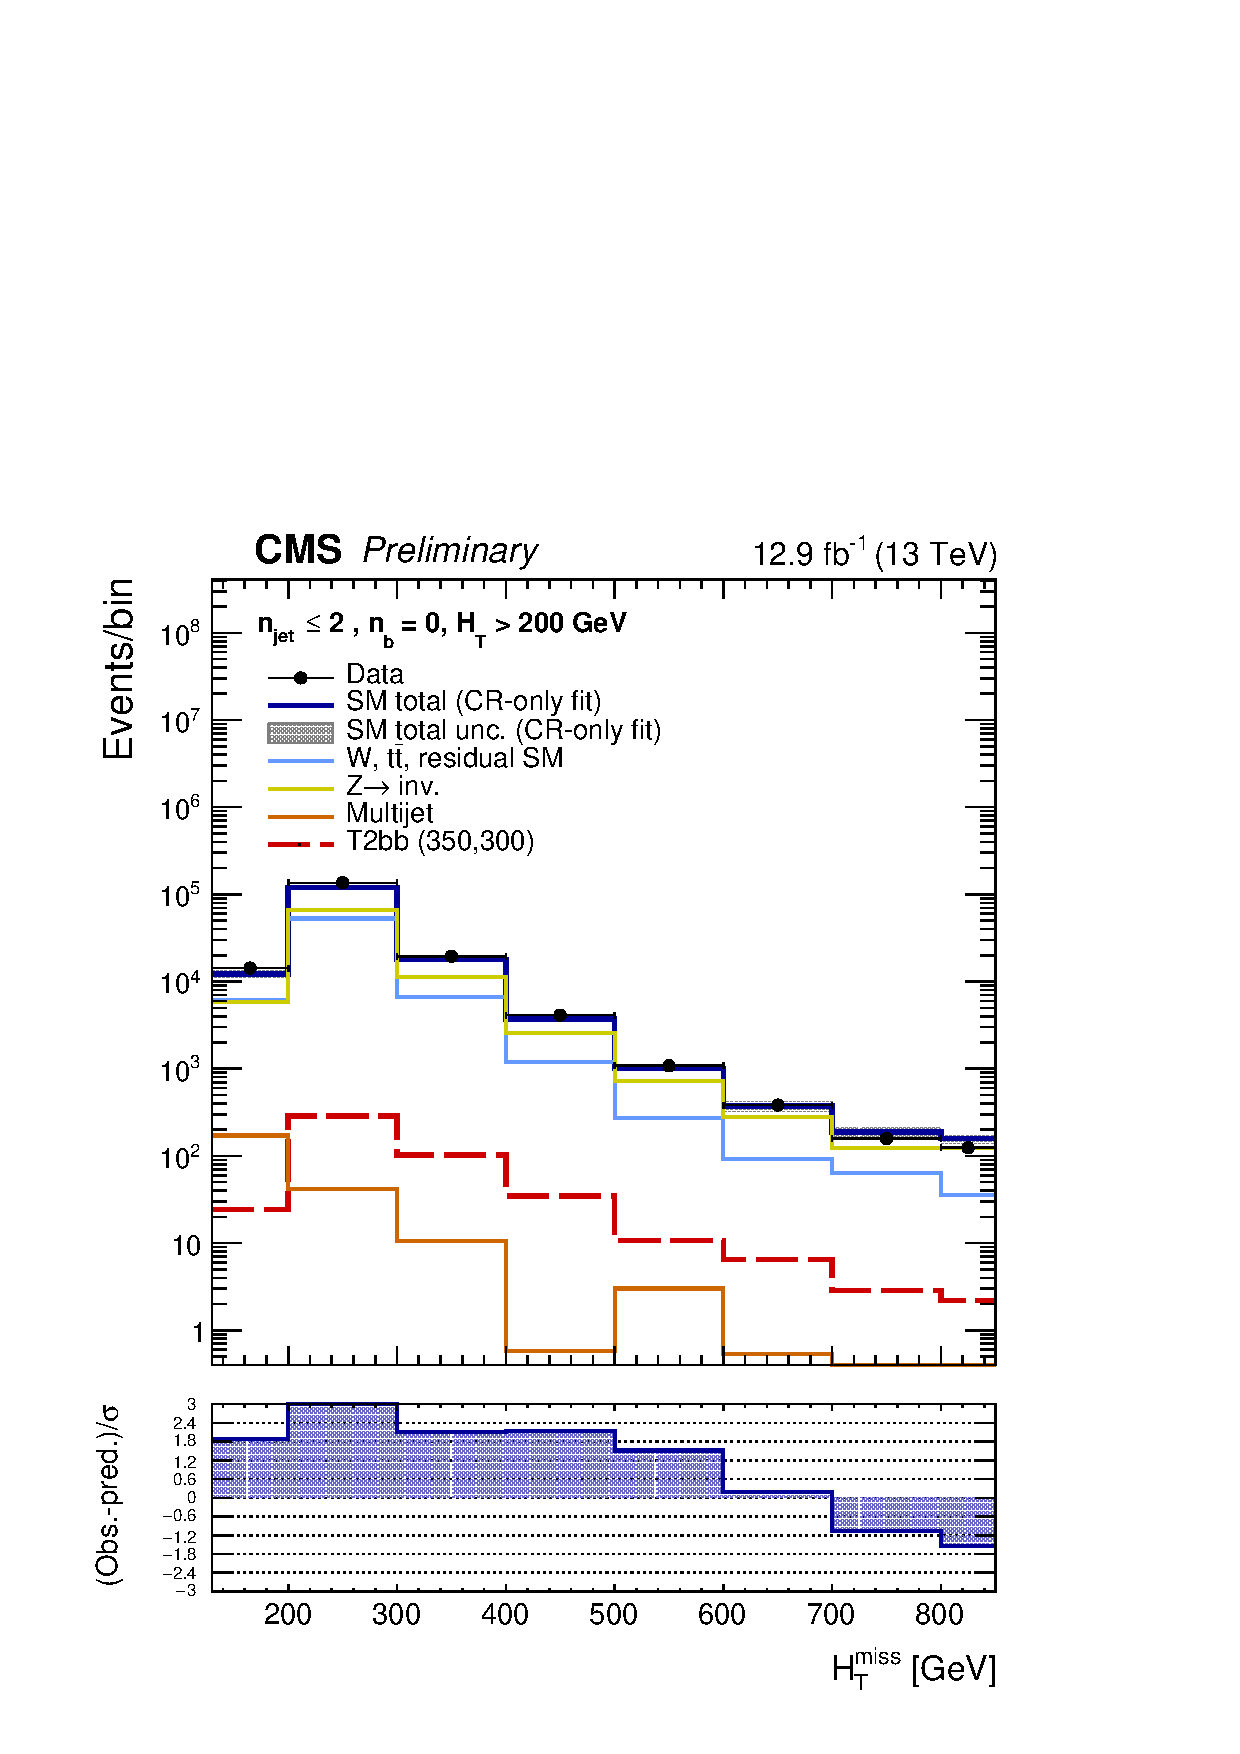
\includegraphics[width=0.4\textwidth]{figures/agg_fitResults/mhtShape_eq0b_le2j_200_Inf_crfit_aux.pdf} } ~~
    \subfigure[Monojet-like, $\nb \geq 1$]{ 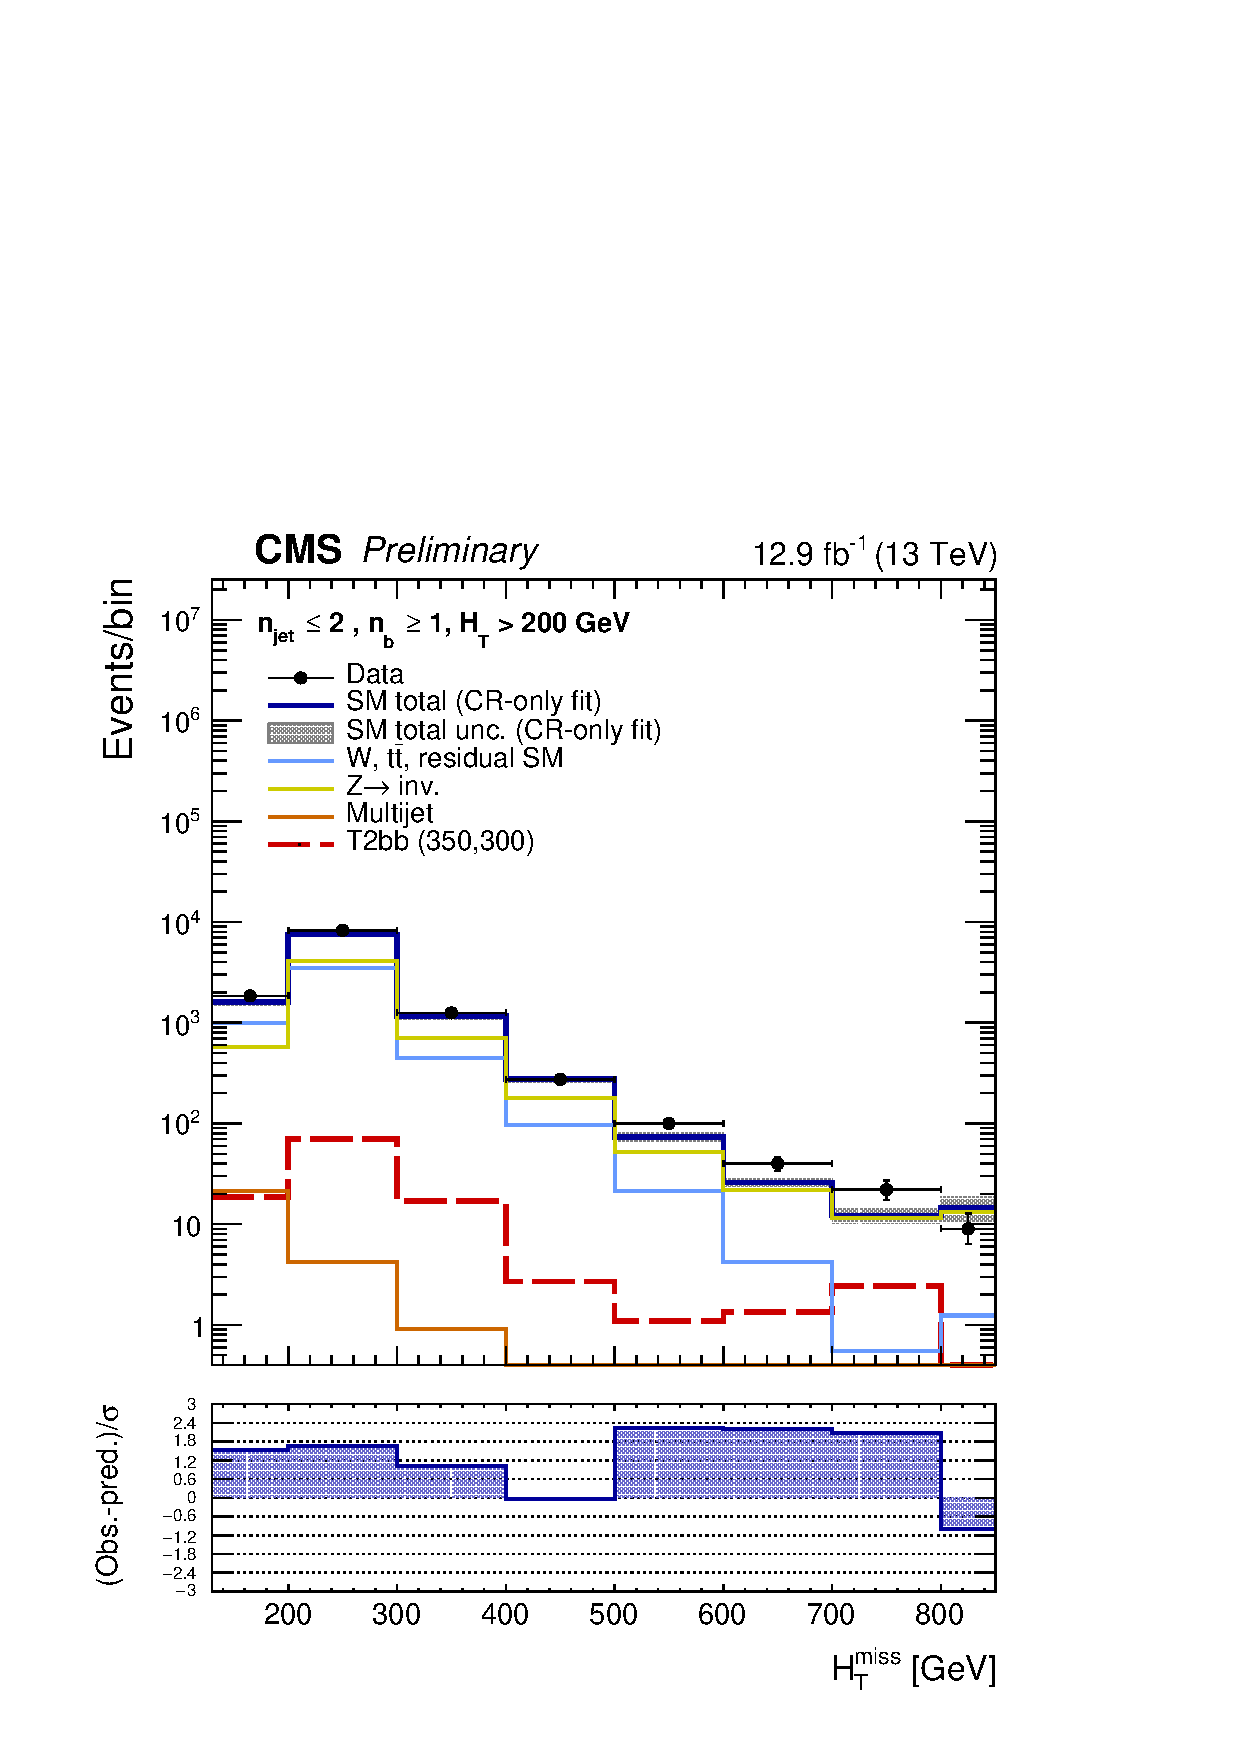
\includegraphics[width=0.4\textwidth]{figures/agg_fitResults/mhtShape_ge1b_le2j_200_Inf_crfit_aux.pdf} } \\
    \subfigure[Asymmetric high \nj, $\nb \leq 1$]   { 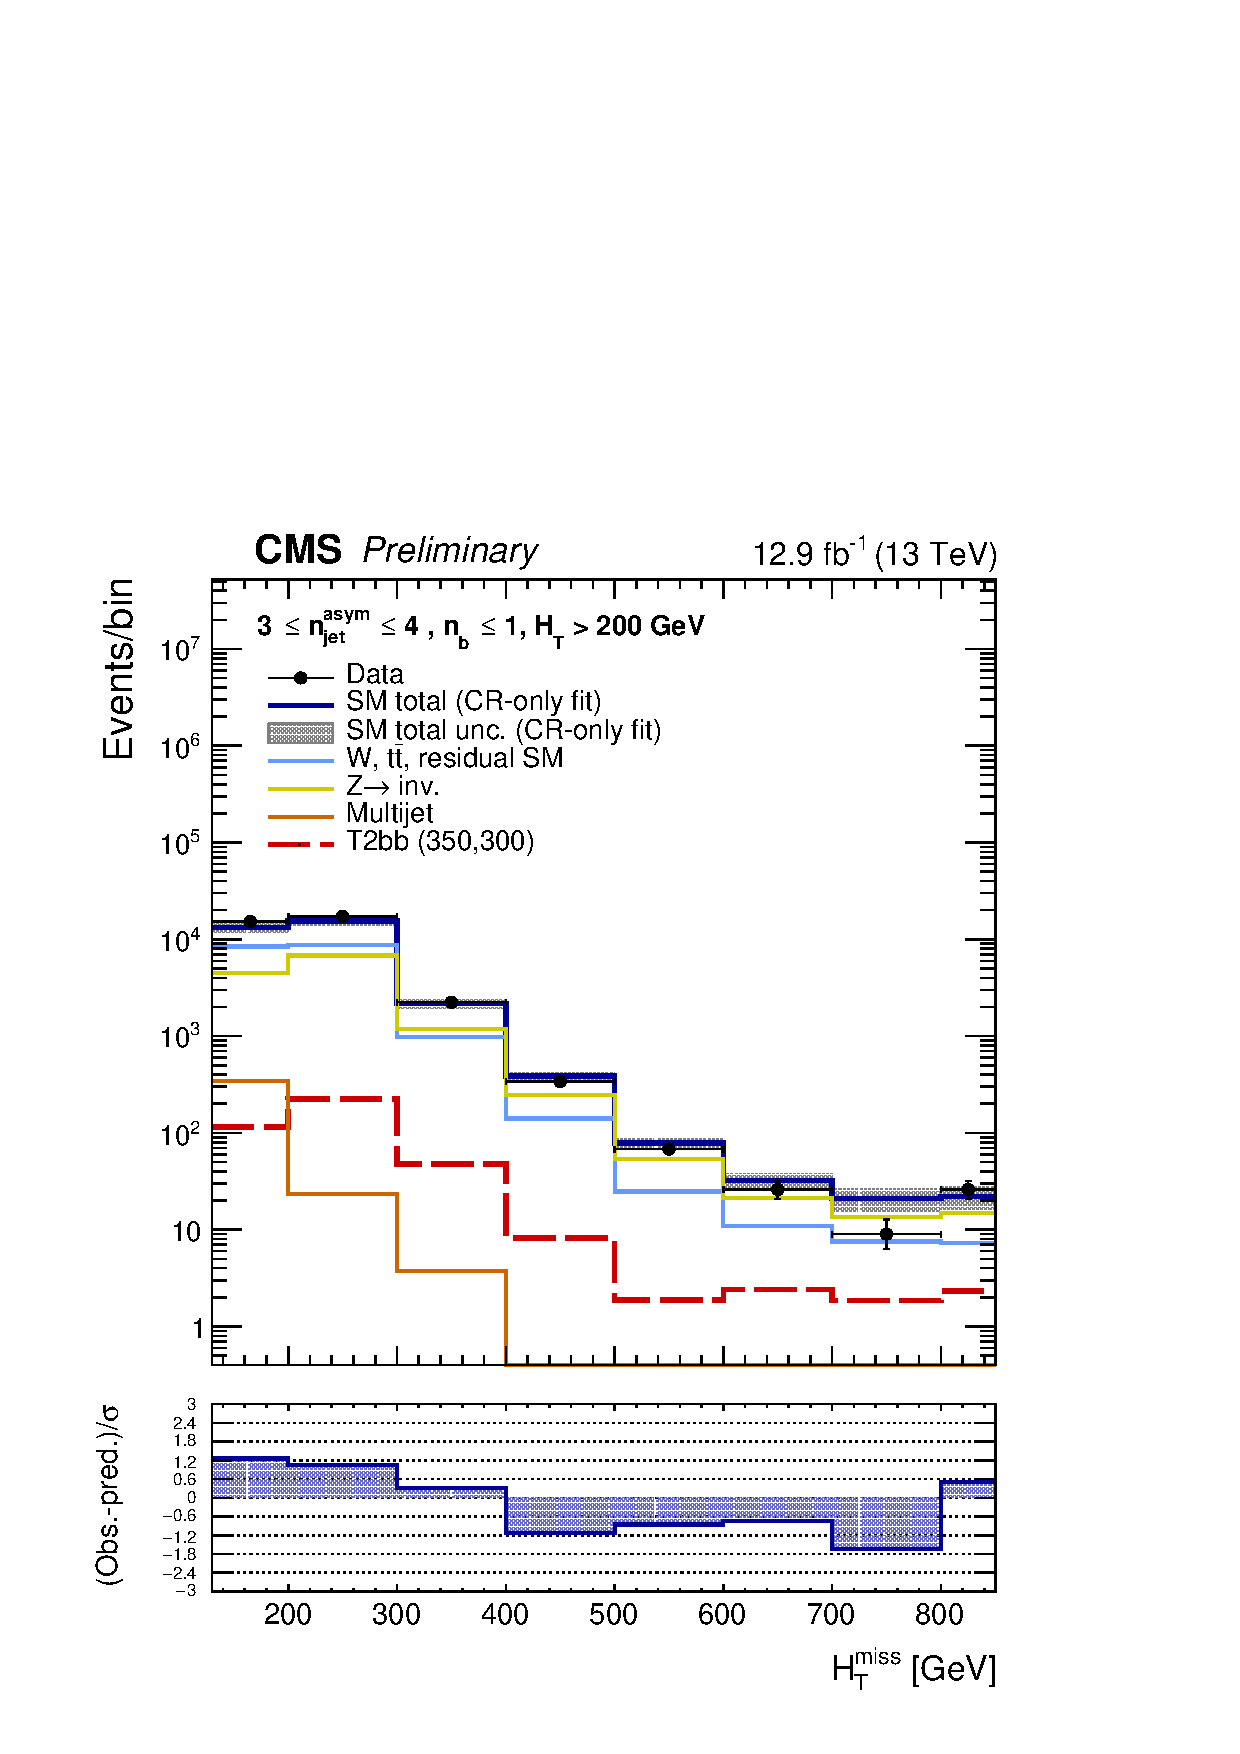
\includegraphics[width=0.4\textwidth]{figures/agg_fitResults/mhtShape_le1b_ge3a_200_Inf_crfit_aux.pdf} } ~~
    \subfigure[Asymmetric high \nj, $\nb \geq 2$]{ 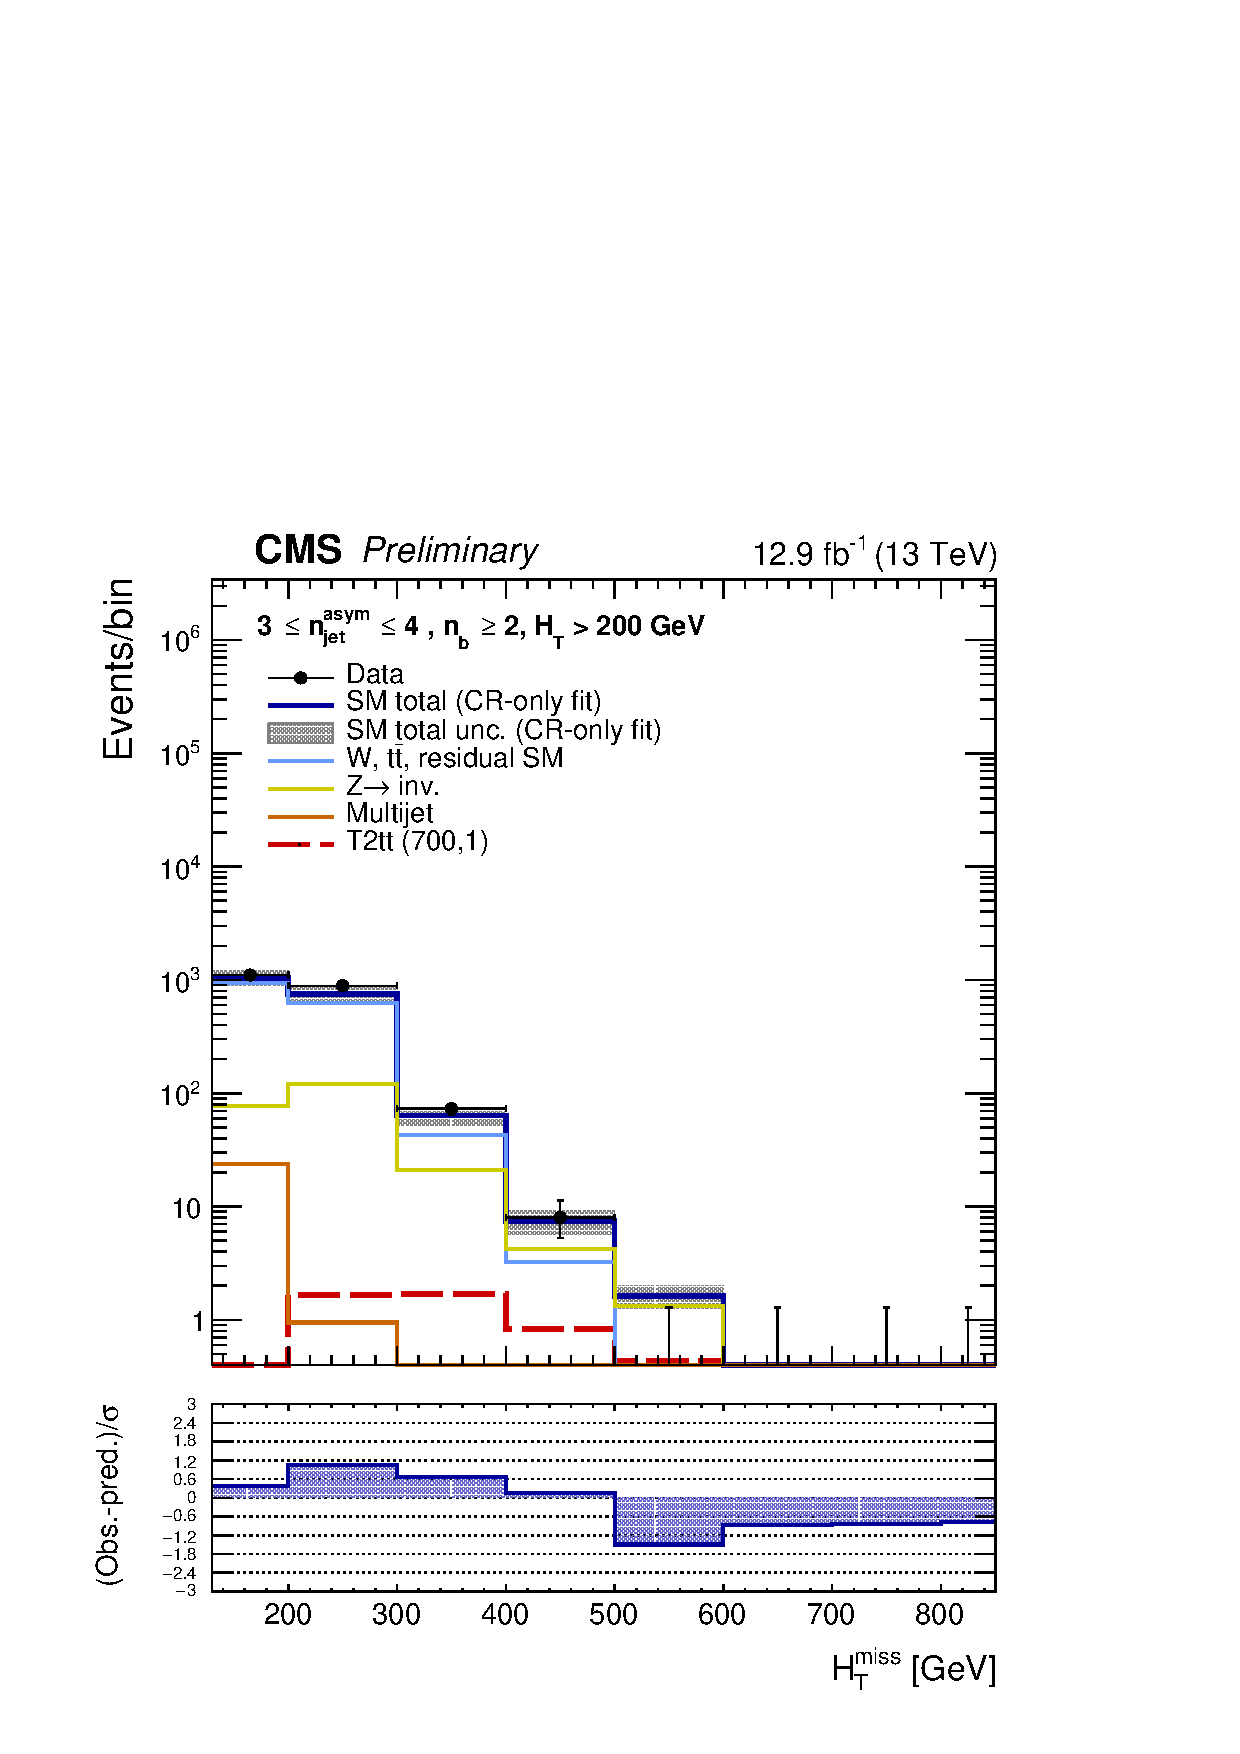
\includegraphics[width=0.4\textwidth]{figures/agg_fitResults/mhtShape_ge2b_ge3a_200_Inf_crfit_aux.pdf} } \\
    \subfigure[Mid \nj, $\nb \leq 1$]   { 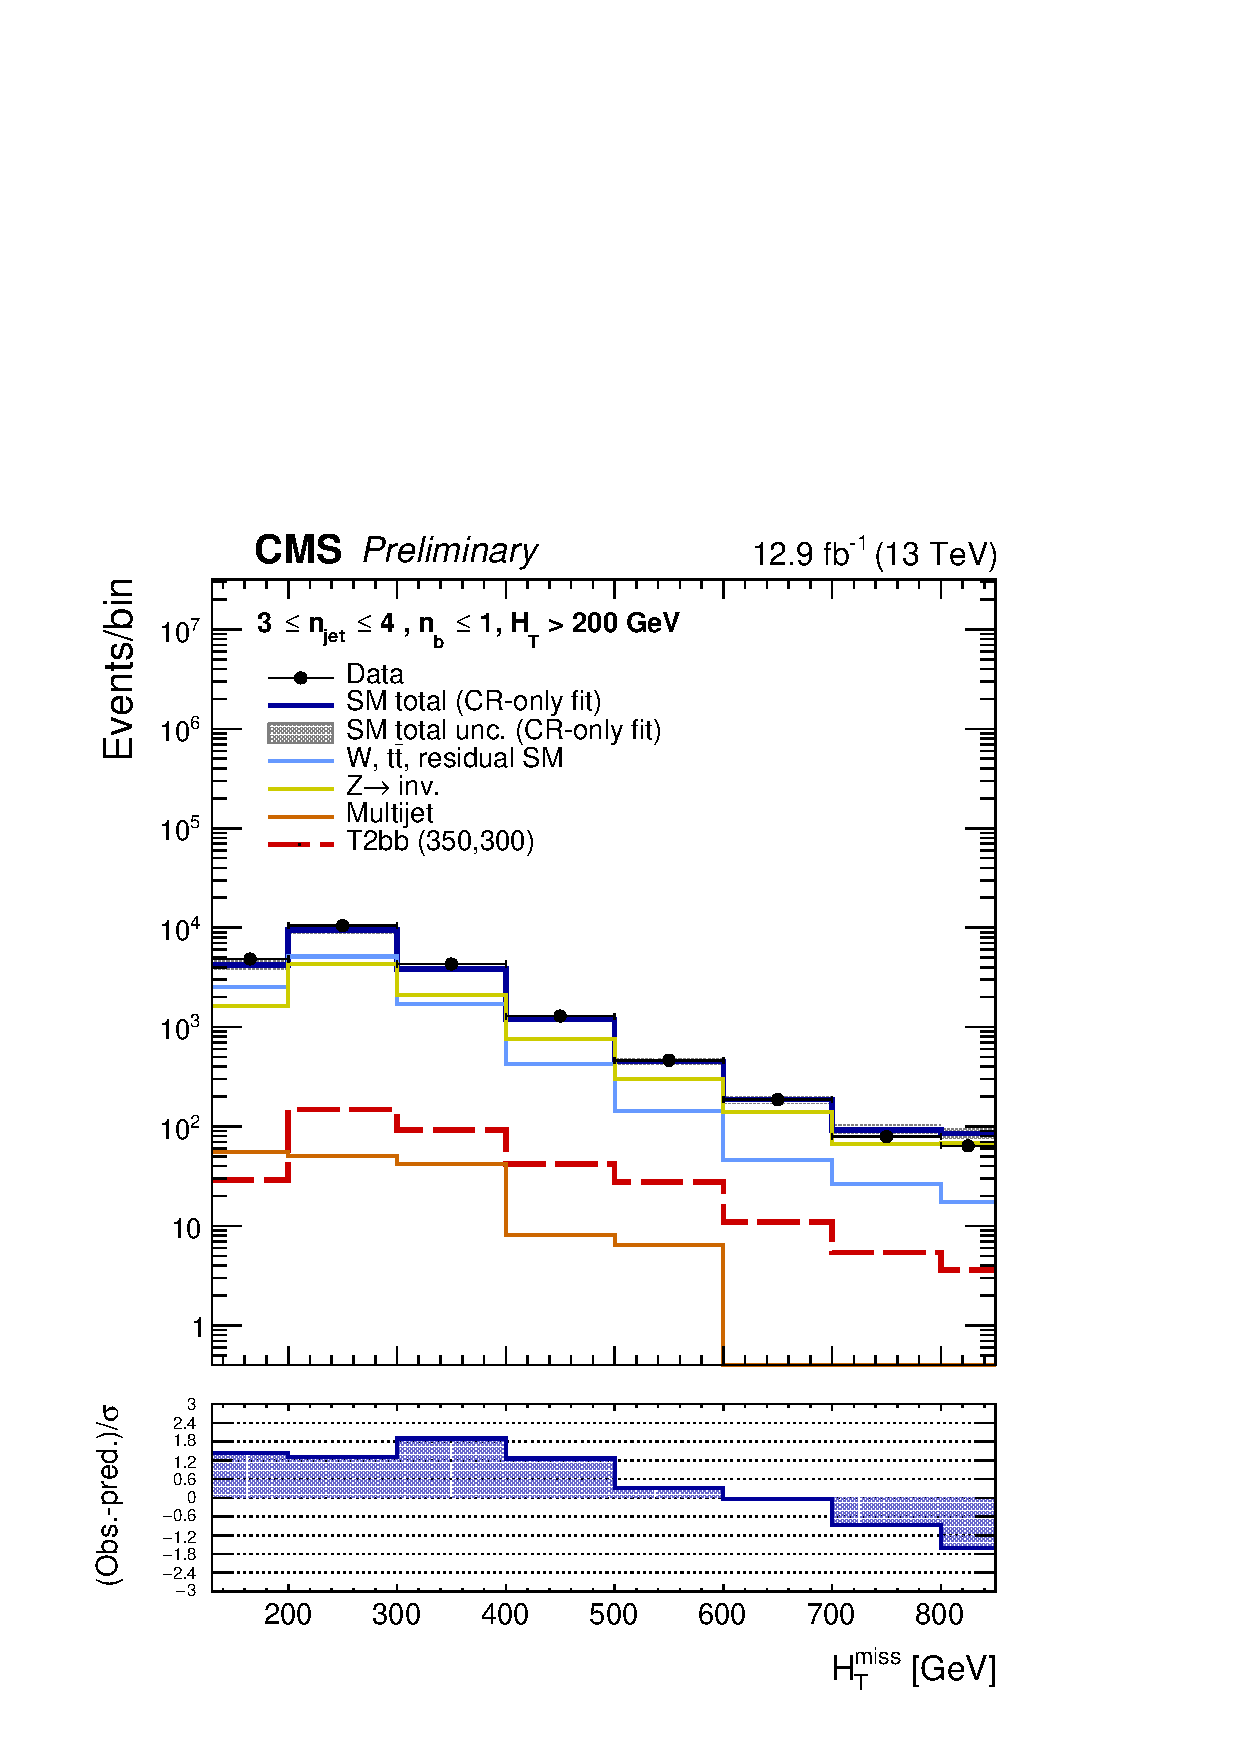
\includegraphics[width=0.4\textwidth]{figures/agg_fitResults/mhtShape_le1b_ge3j_200_Inf_crfit_aux.pdf} } ~~
    \subfigure[Mid \nj, $\nb \geq 2$]{ 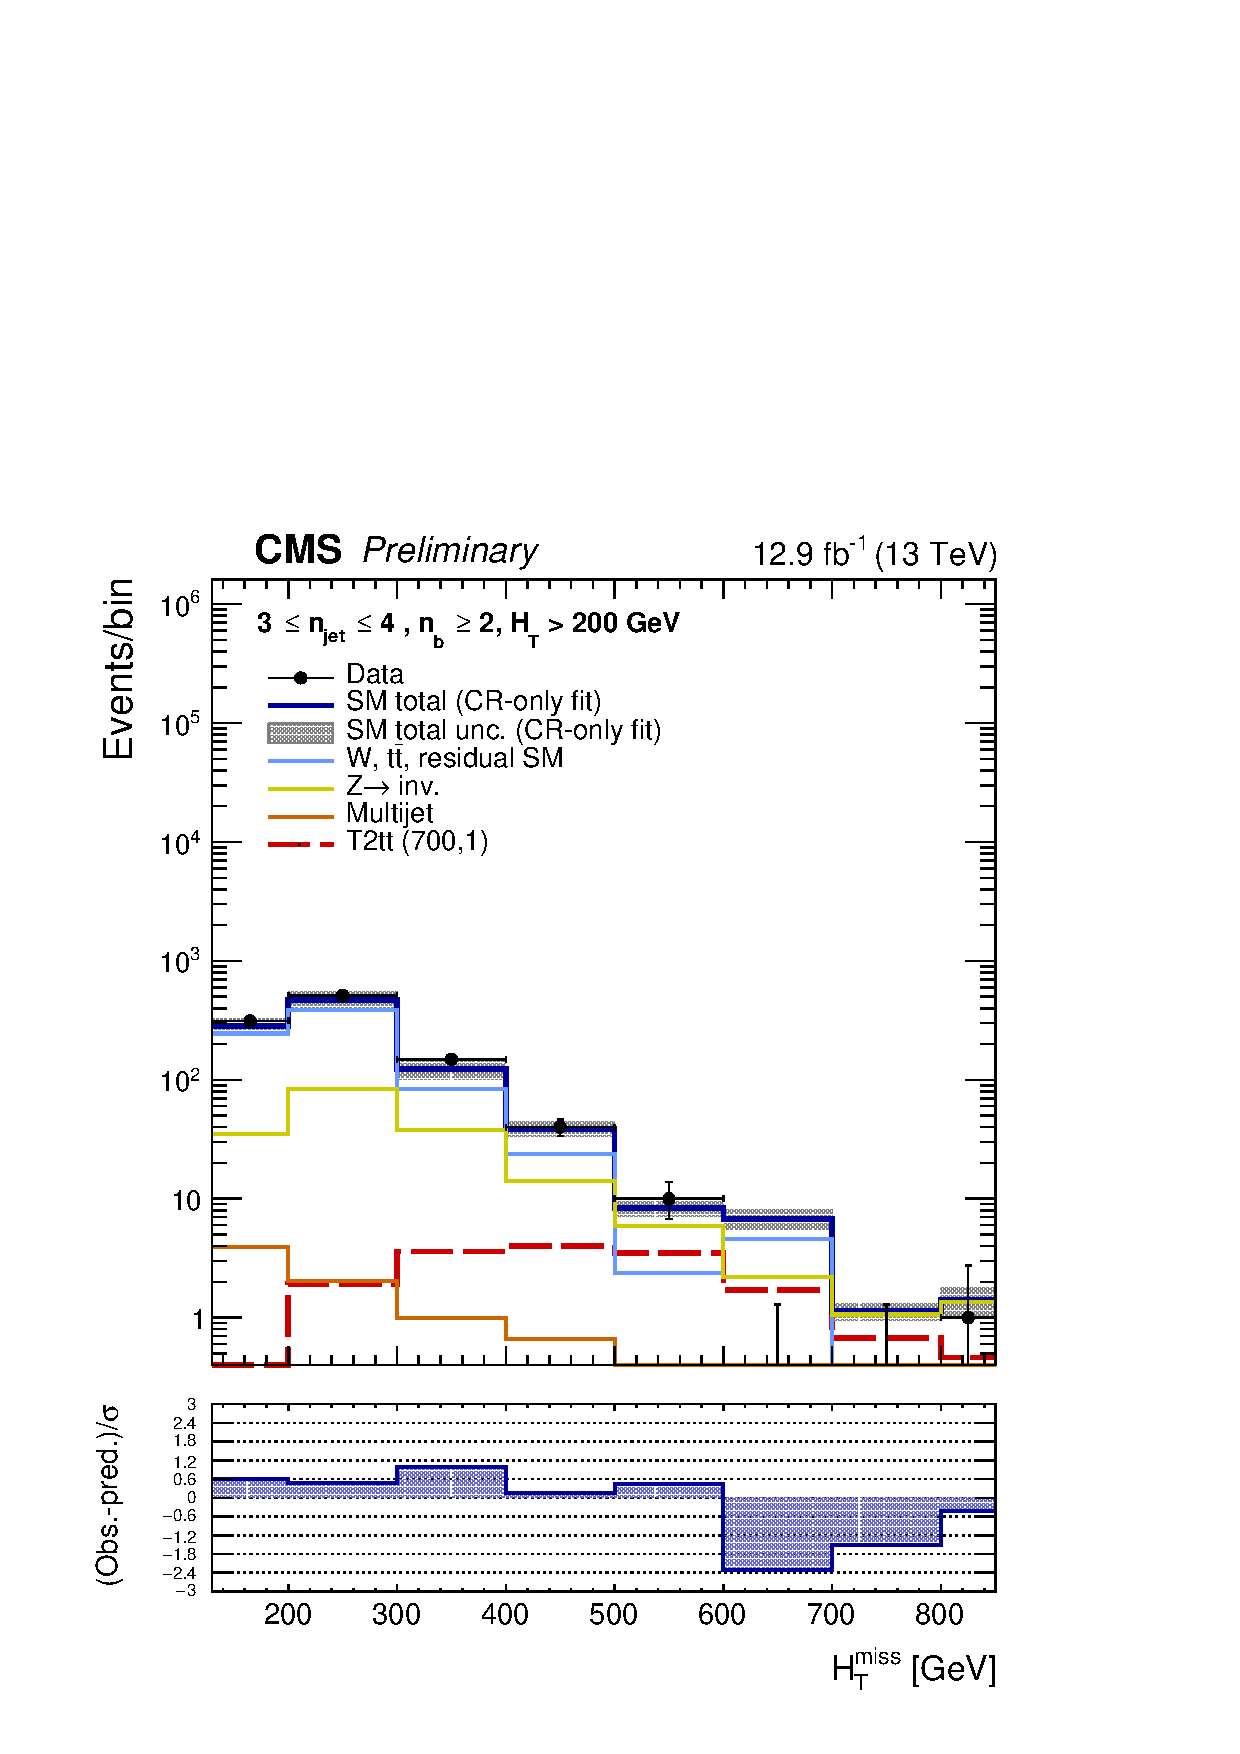
\includegraphics[width=0.4\textwidth]{figures/agg_fitResults/mhtShape_ge2b_ge3j_200_Inf_crfit_aux.pdf} } \\
    \subfigure[High \nj, $\nb \leq 1$]   { 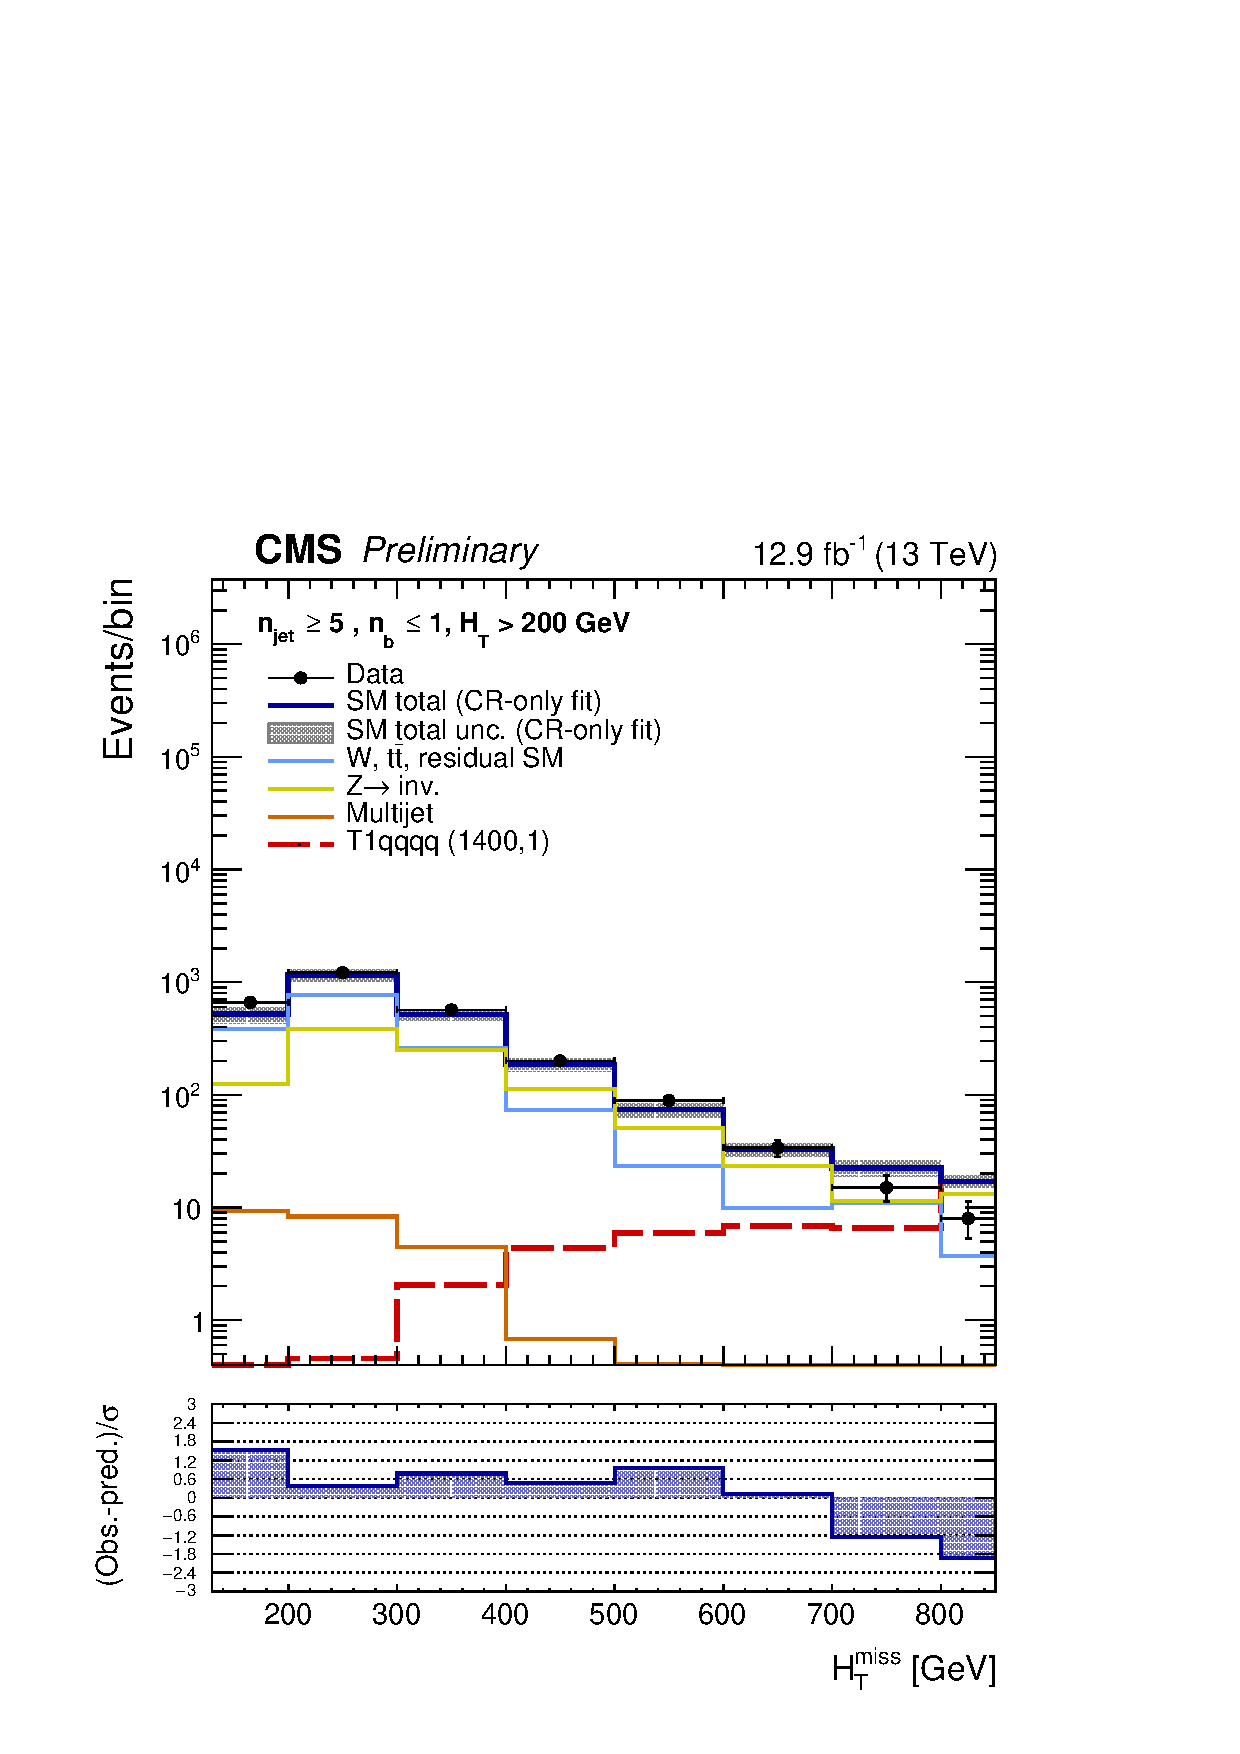
\includegraphics[width=0.4\textwidth]{figures/agg_fitResults/mhtShape_le1b_ge5j_200_Inf_crfit_aux.pdf} } ~~
    \subfigure[High \nj, $\nb \geq 2$]{ 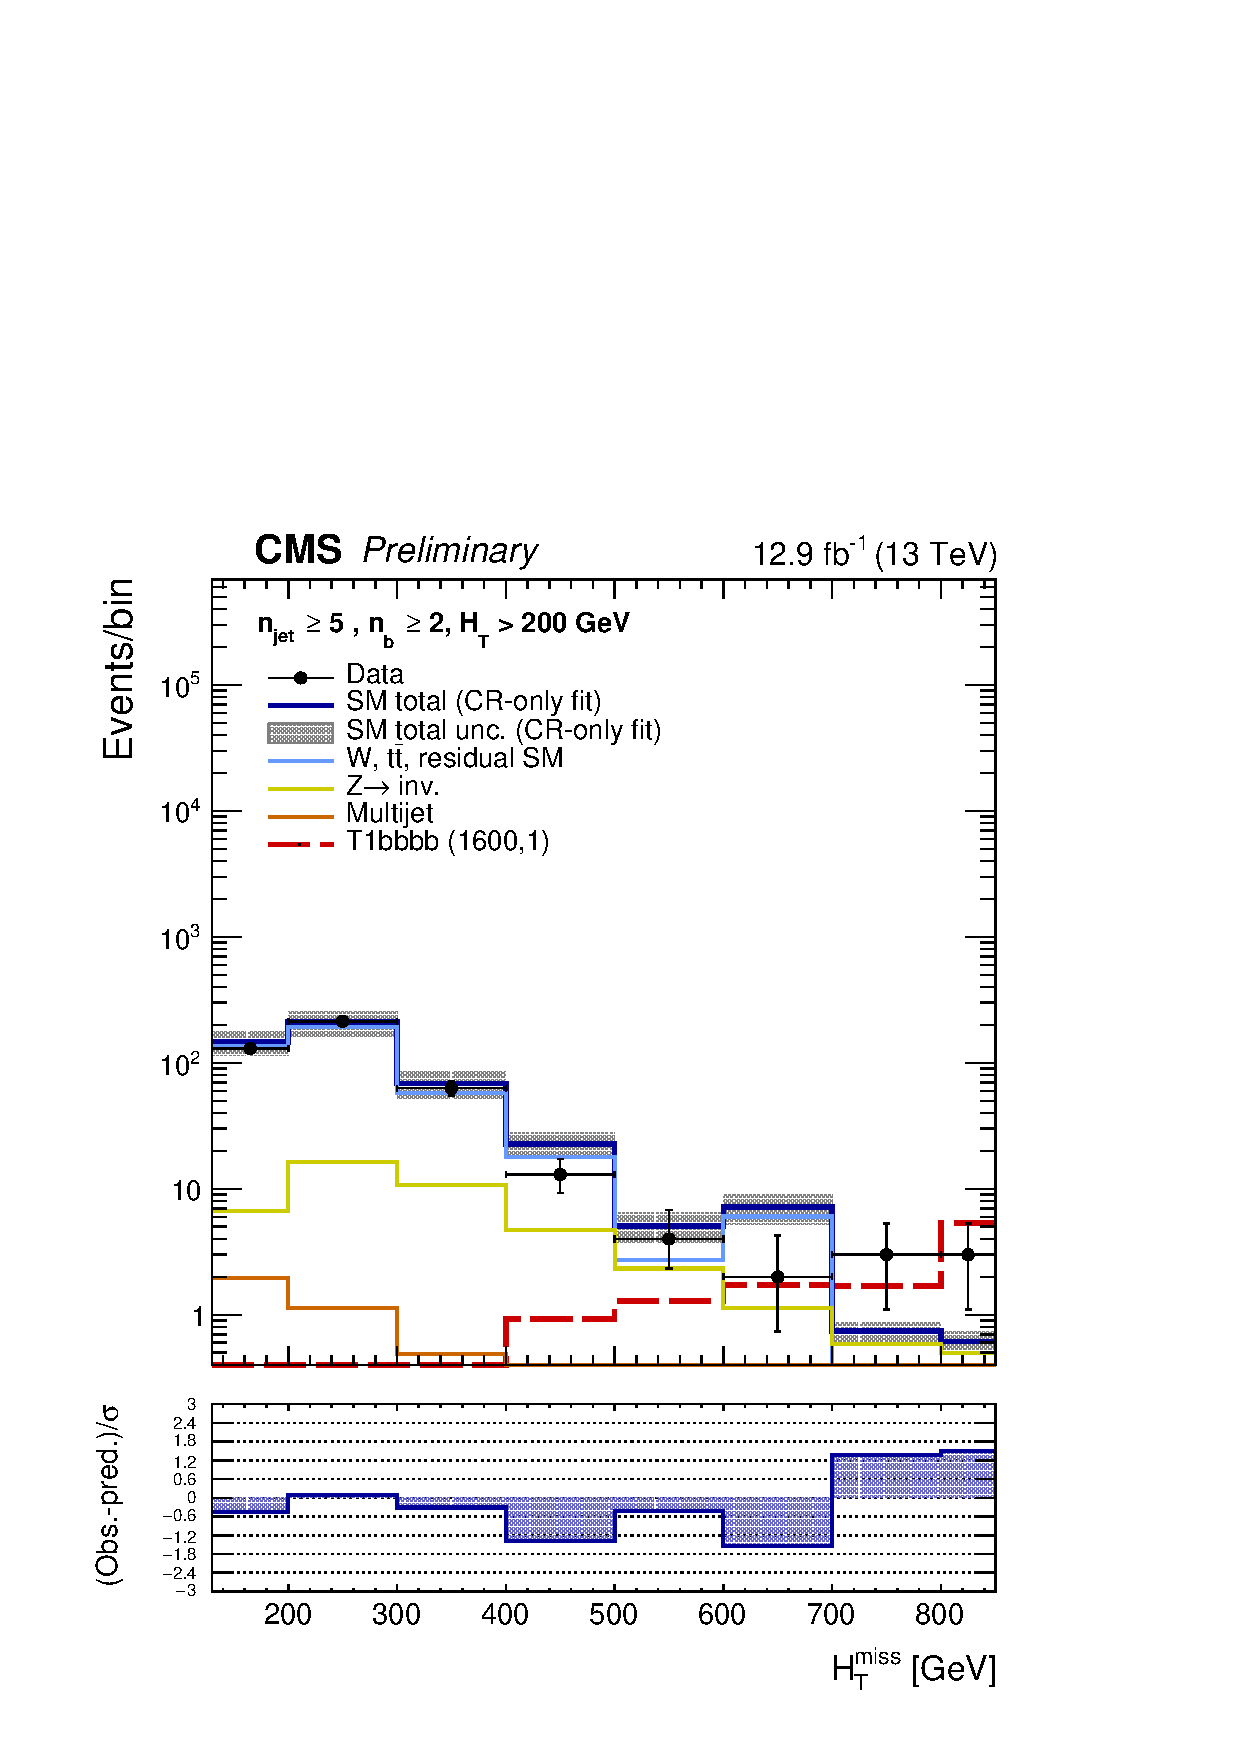
\includegraphics[width=0.4\textwidth]{figures/agg_fitResults/mhtShape_ge2b_ge5j_200_Inf_crfit_aux.pdf} } \\
  \end{center}
\end{figure}


\clearpage
\begin{figure}[!tbhp]
    \caption{ Limit planes shown for both the full signal regions (left) and the aggregate regions (right).\label{fig:limit-planes}. 
    For the compressed models. }
  \begin{center}
    \subfigure[T2bb full signal region]{ 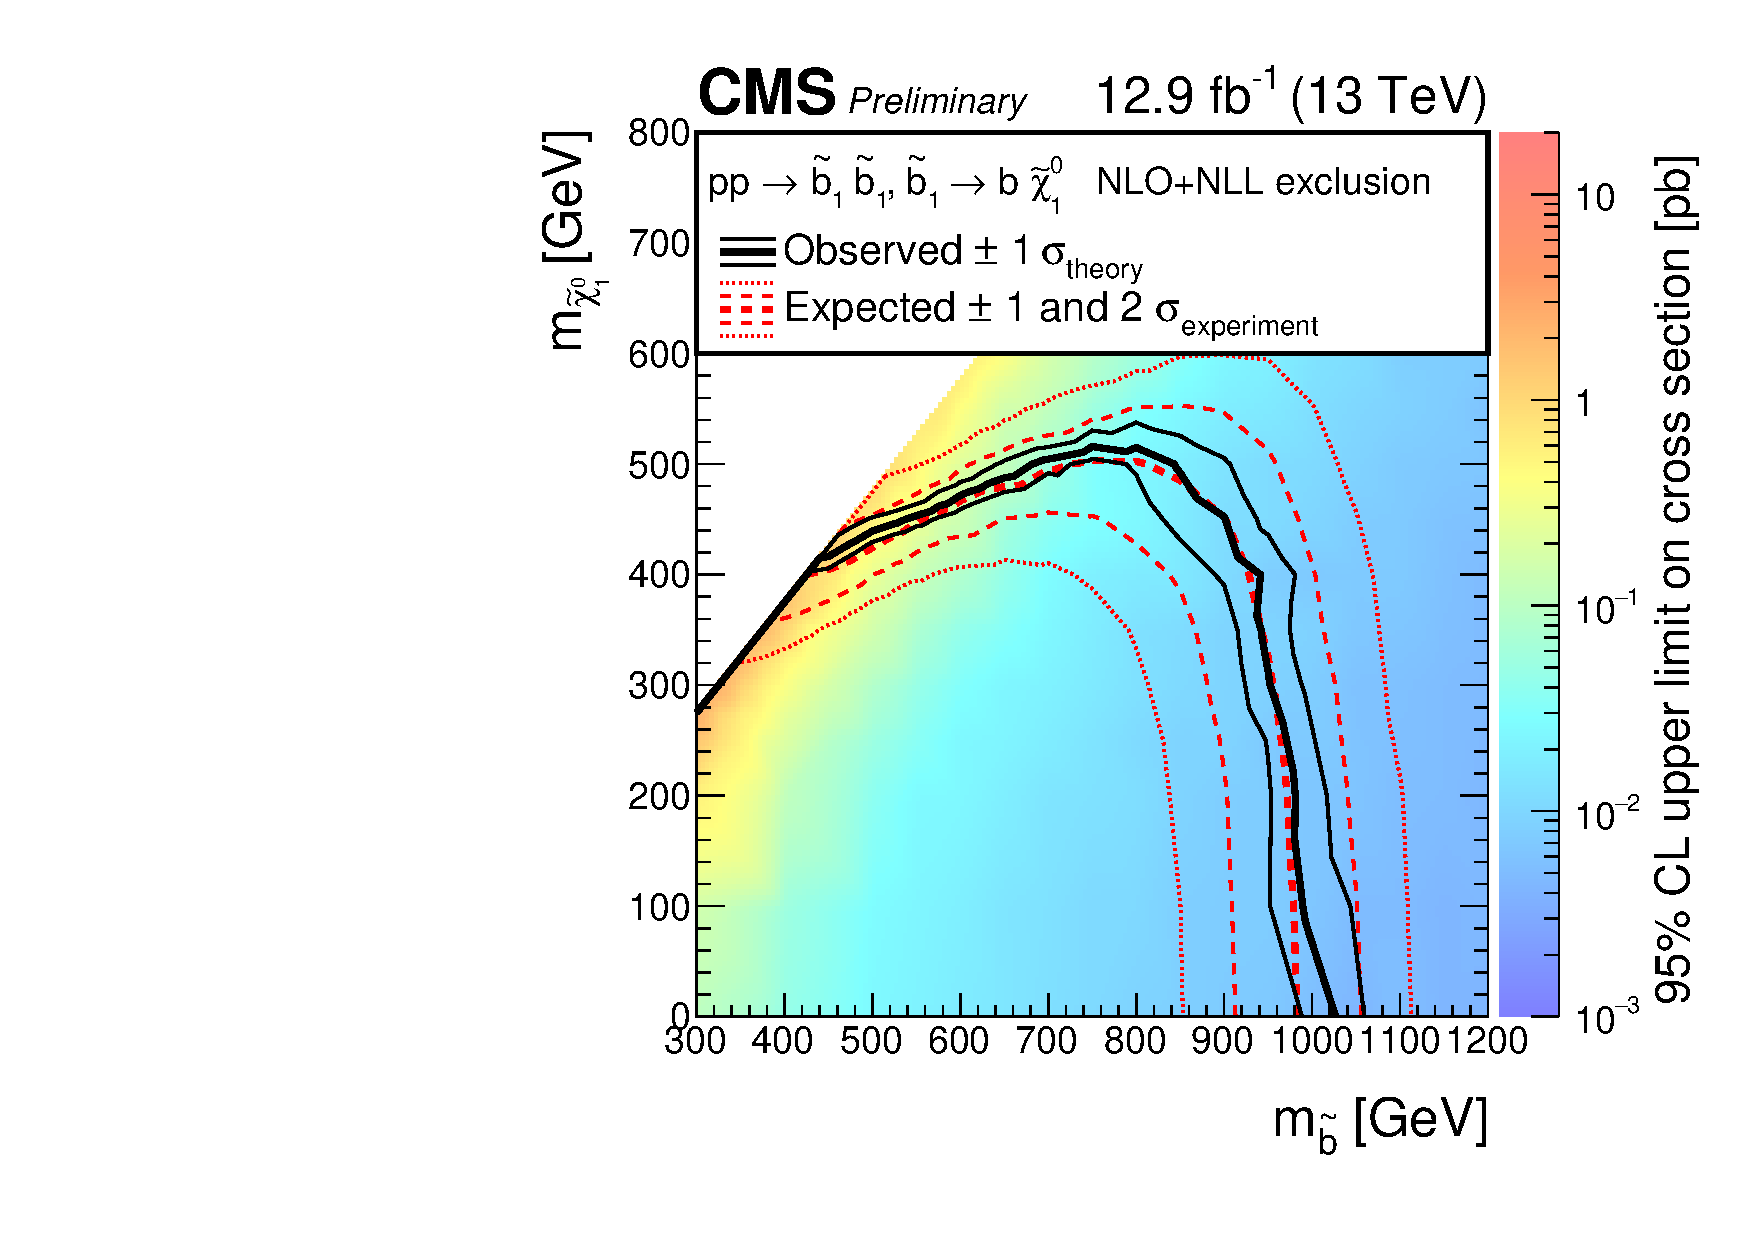
\includegraphics[width=0.45\textwidth]{figures/limitPlanesNominal/SUS16T2bbXSEC} } ~~
    \subfigure[T2bb aggregate regions]{ 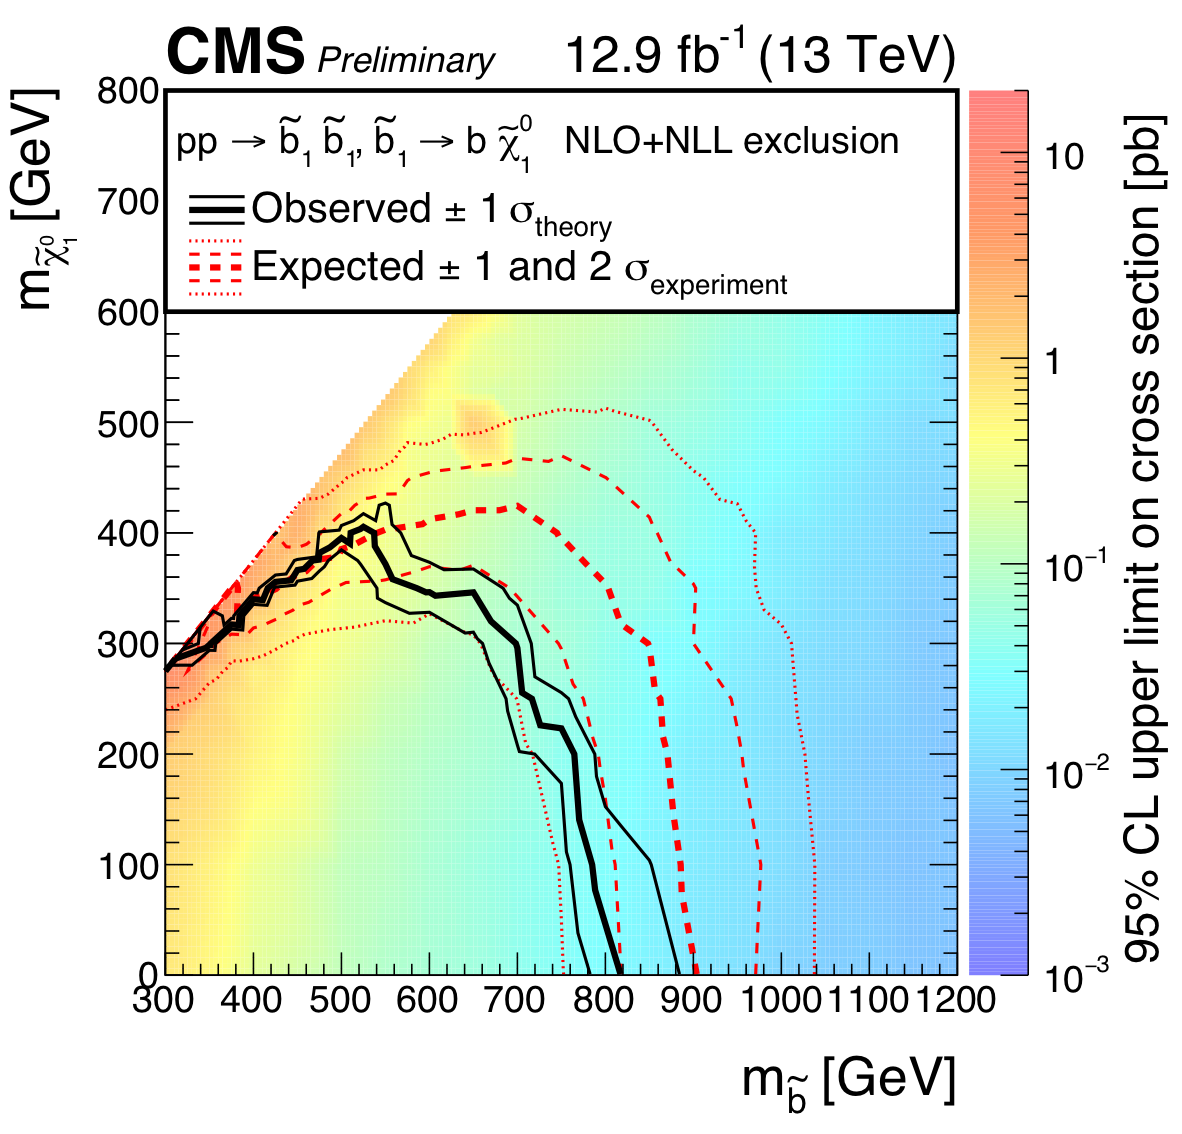
\includegraphics[width=0.45\textwidth]{figures/limitPlanesAgg/SUS16T2bbXSEC} } \\
    \subfigure[T2tt full signal region]   { 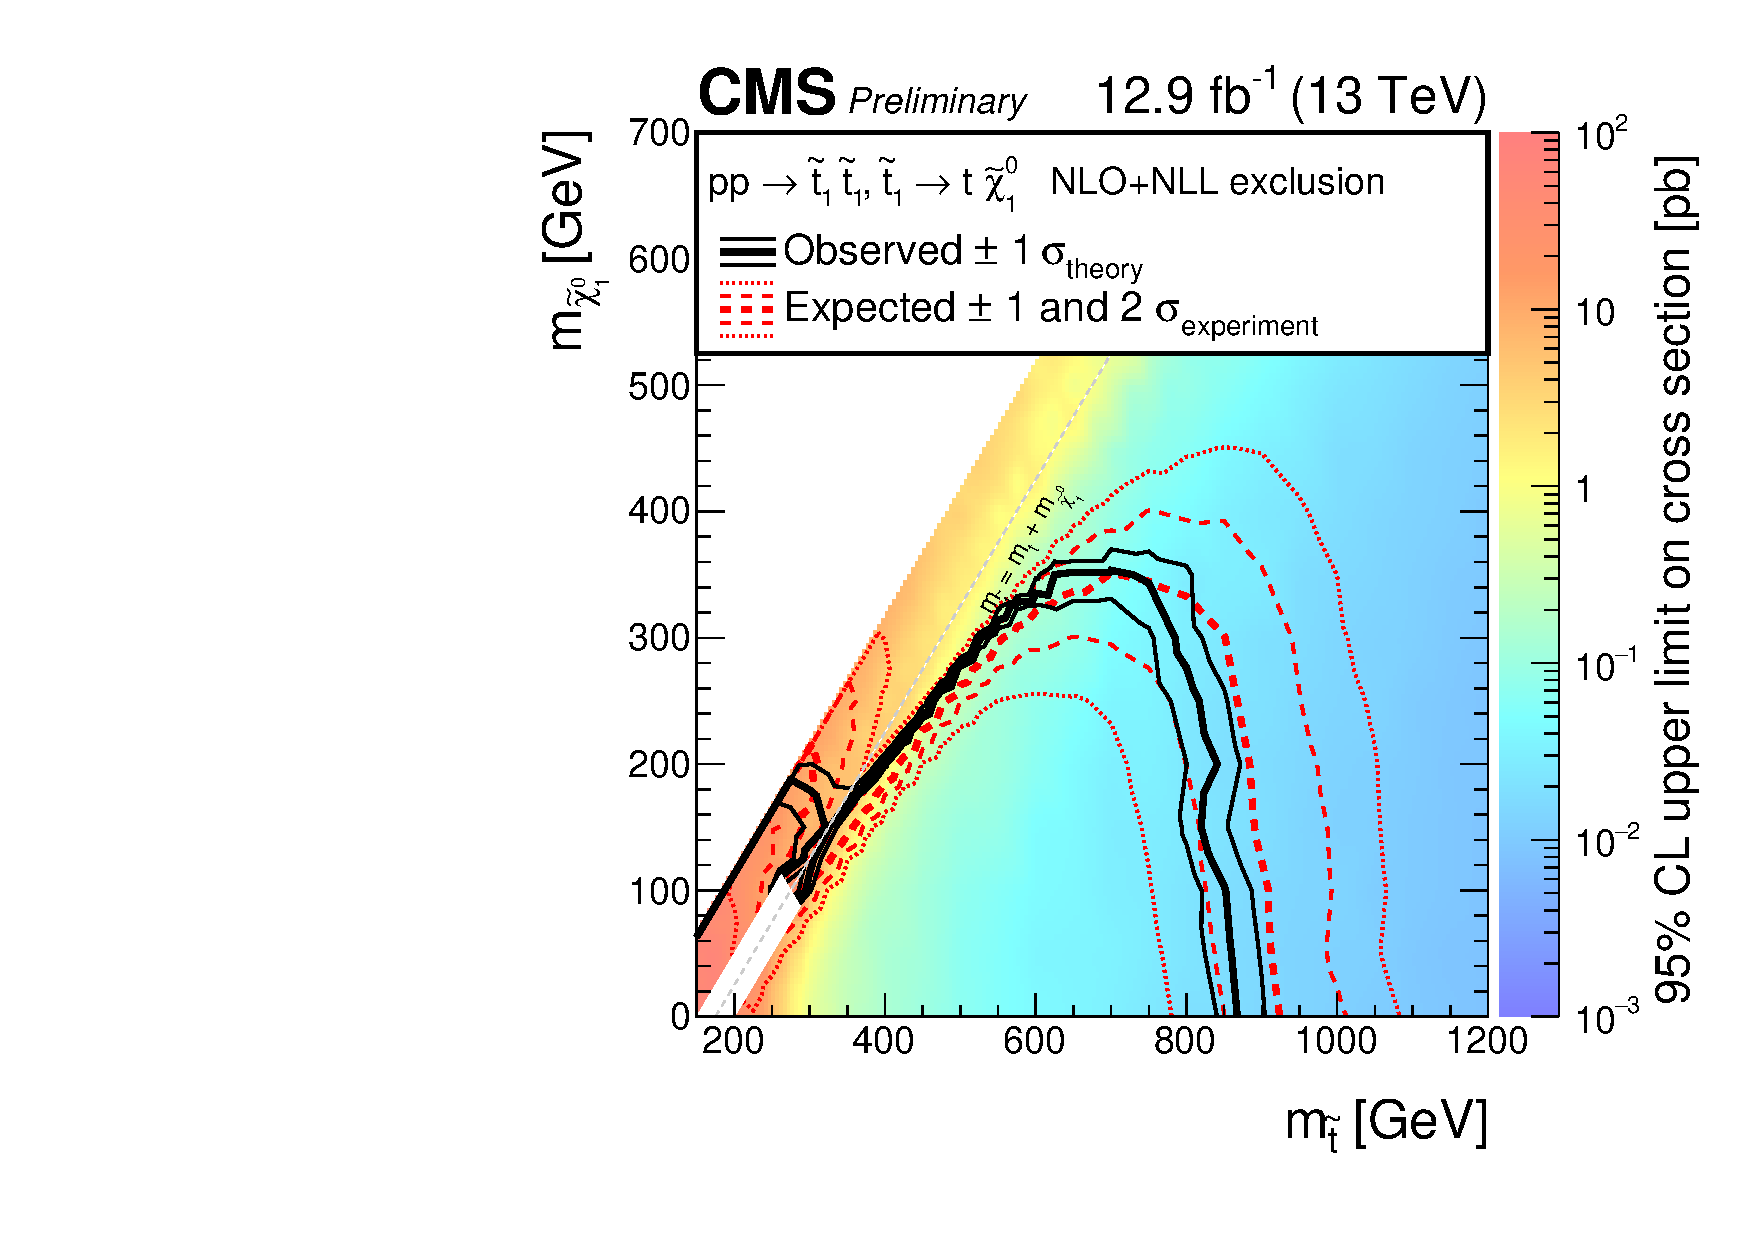
\includegraphics[width=0.45\textwidth]{figures/limitPlanesNominal/SUS16T2ttXSEC} } ~~
    \subfigure[T2tt aggregate regions]{ 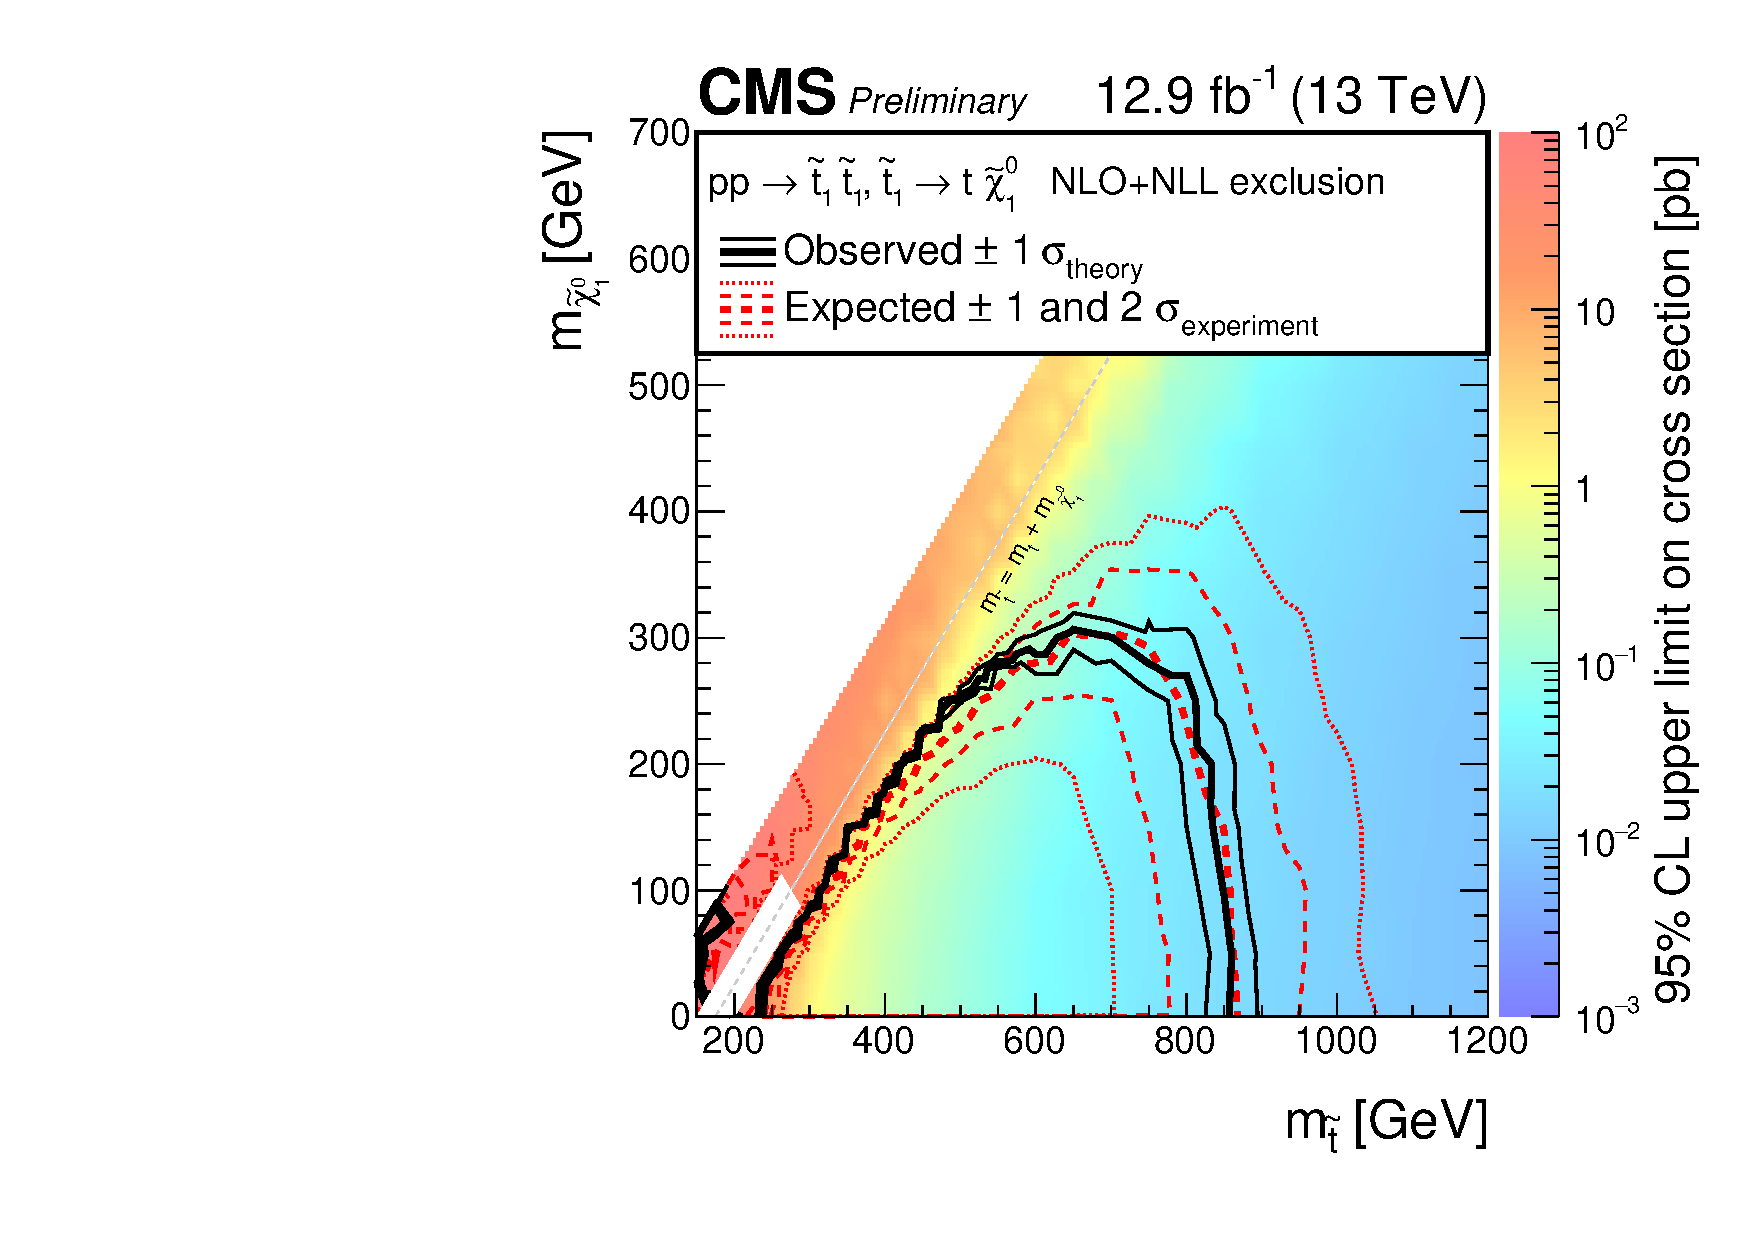
\includegraphics[width=0.45\textwidth]{figures/limitPlanesAgg/SUS16T2ttXSEC} } \\
    \subfigure[T1bbbb full signal region]   { 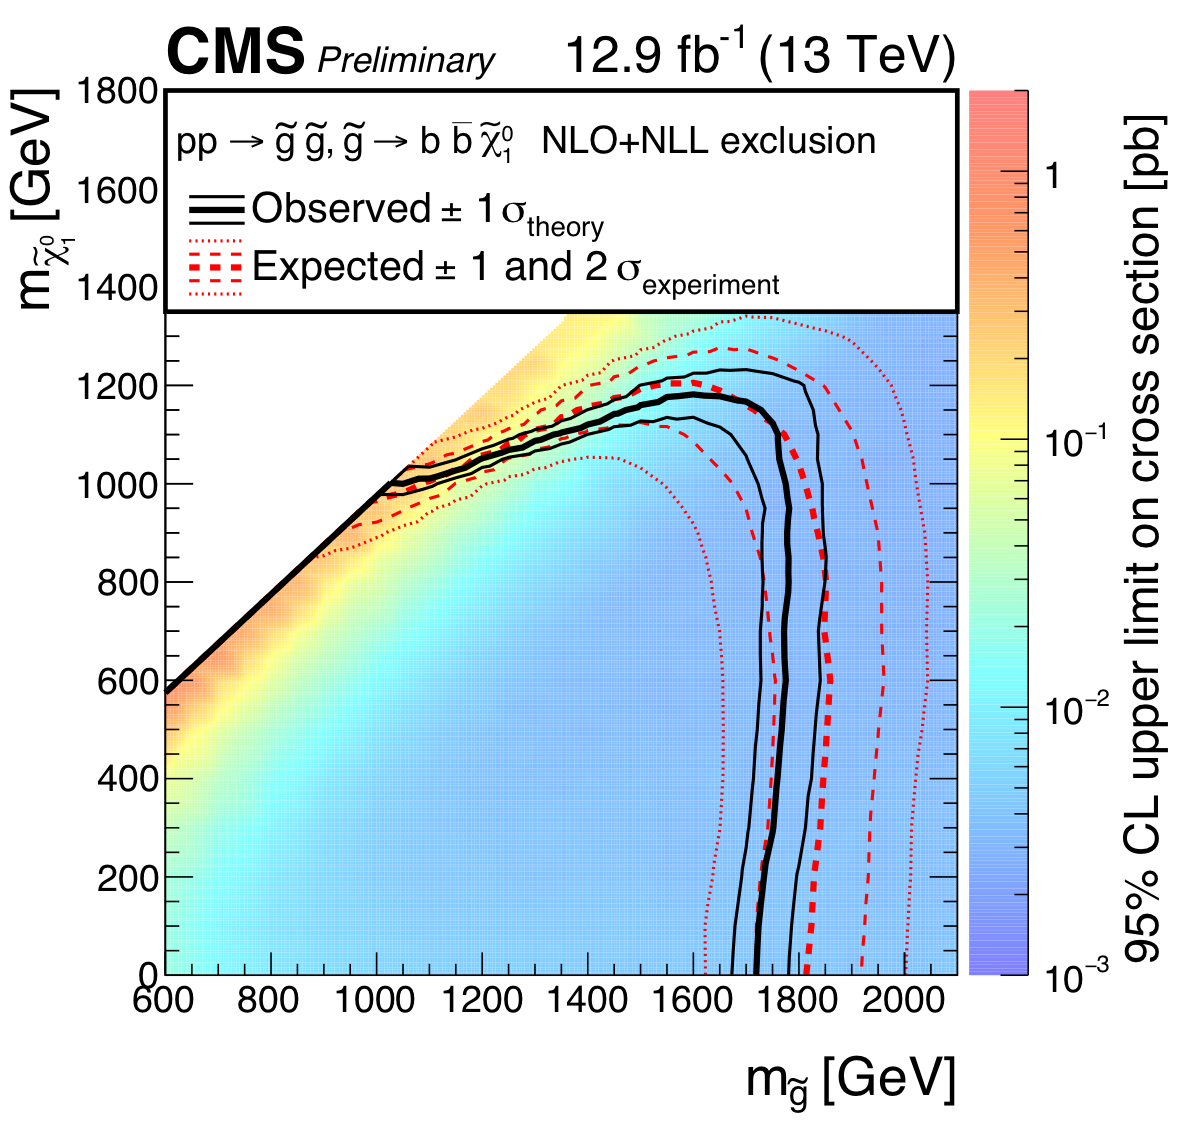
\includegraphics[width=0.45\textwidth]{figures/limitPlanesNominal/SUS16T1bbbbXSEC} } ~~
    \subfigure[T1bbbb aggregate regions]{ 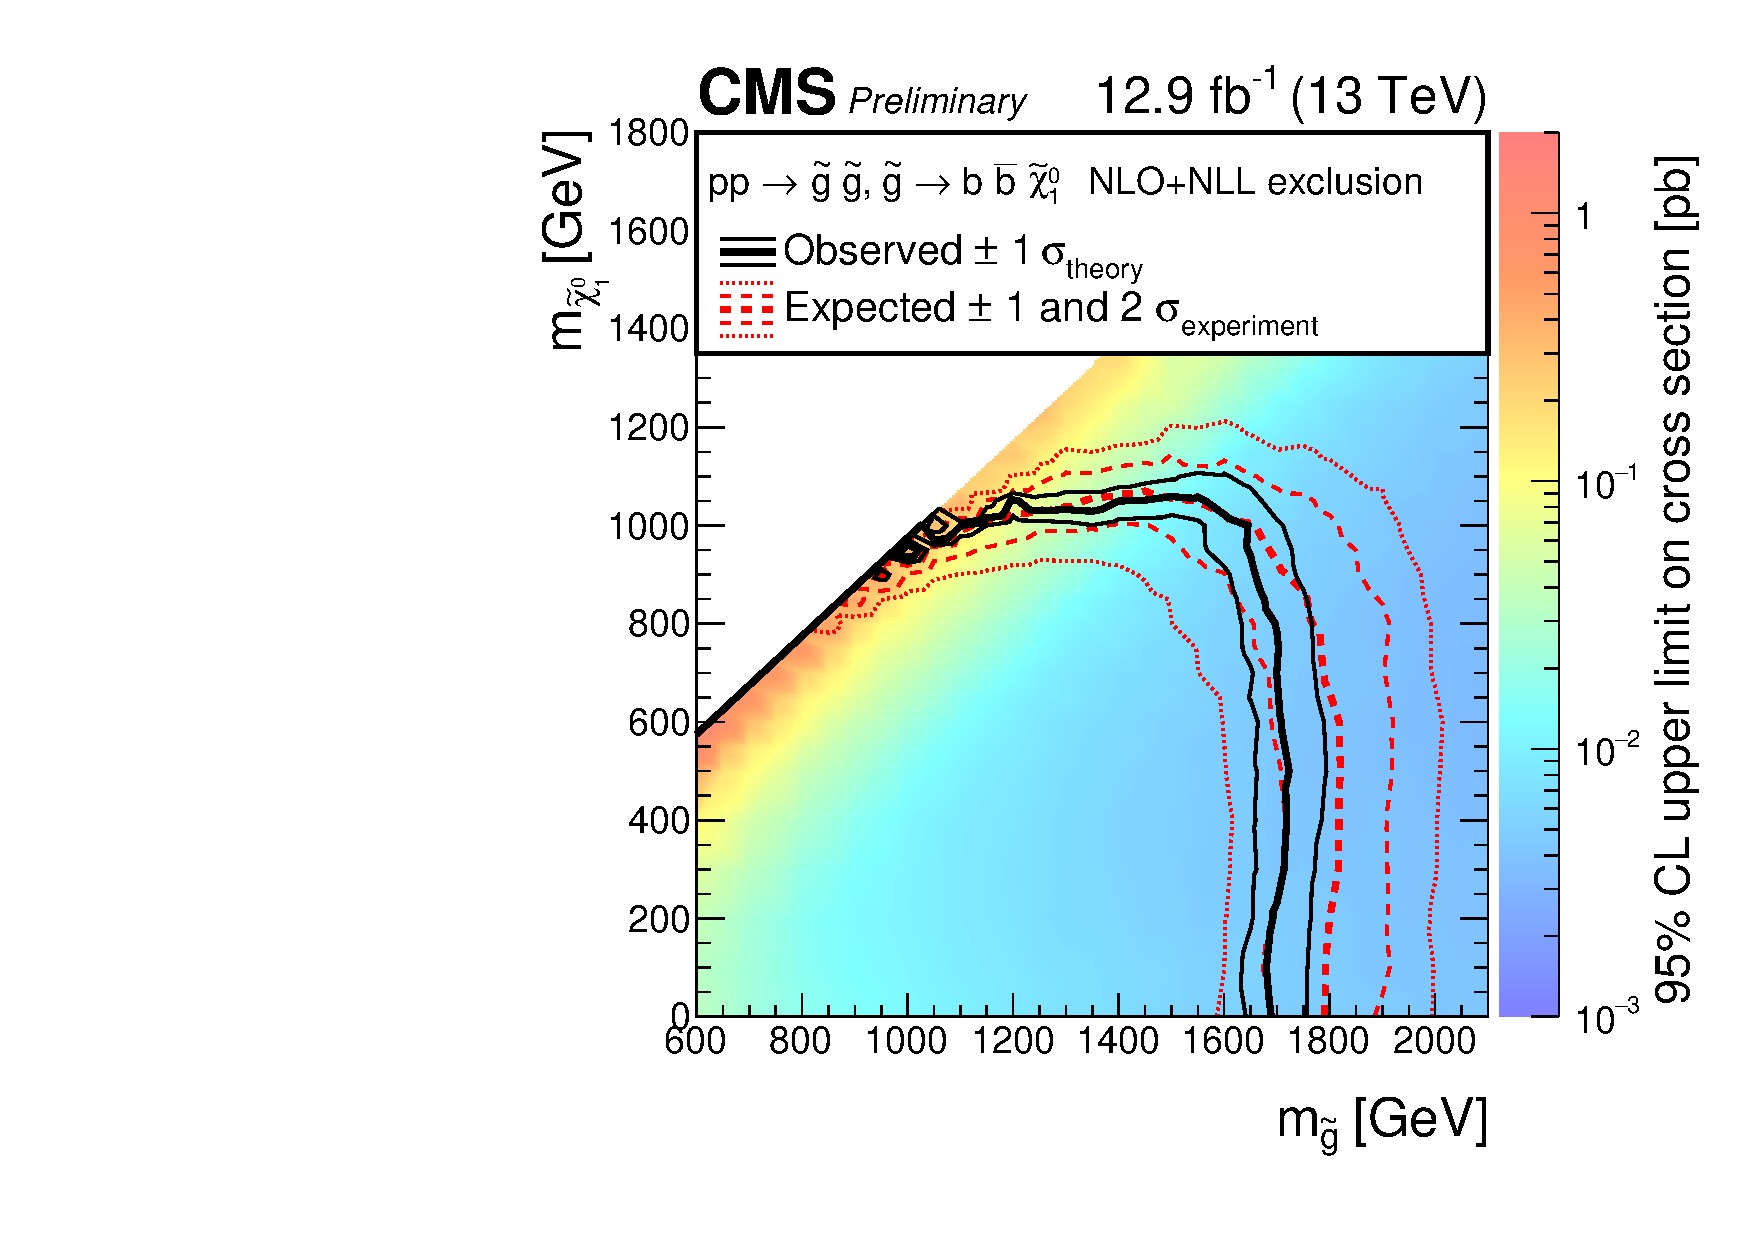
\includegraphics[width=0.45\textwidth]{figures/limitPlanesAgg/SUS16T1bbbbXSEC} } \\
  \end{center}
\end{figure}
%%____________________________________________________________________________||



%%____________________________________________________________________________||
\section{Simplified likelihood}
\label{sec:simplified-likelihood}

This section describes a procedure for using the information provided by the CMS Collaboration to 
re-interpret searches for new physics through the use of a simplified likelihood. The likelihood is 
constructed from a product of counting experiments, representing each search bin in one or more search regions. 
For a given bin, $i$, the probability to observe $n_{i}$ events is given by

\begin{equation}
 P_{i}(\mu) := P(d_{i}|\mu \cdot s_{i}+b_{i}) = \dfrac{(\mu \cdot s_{i}+b_{i})^{n_{i}} e^{-(\mu \cdot s_{i}+b_{i})} }{n_{i}!}
\label{eq:poisson-likelihood}
\end{equation}

where $s_{i}$ and $b_{i}$ are the total expected signal and background contributions. 
The likelihood for a search containing $N$ search regions is constructed as the product 
of the probabilities across the $N$ search regions, 

\begin{equation}
\mathcal{L}(\mu) = \prod_{i=1}^{N} P_{i}(\mu)
\label{eq:stat-likelihood}
\end{equation}

In most cases, the background contribution in each search region will not be known with perfect accuracy and is therefore 
subject to systematic uncertainties. These uncertainties are modelled by modifying the background contributions as 
$b_{i}\rightarrow b_{i}+\delta b_{i}$, where $\delta b_{i}$ are constrained nuisance parameters. The likelihood then takes the form

\begin{equation}
\mathcal{L}(\mu, \delta \mathbf{b}) = \prod_{i=1}^{N} P_{i}(\mu,\delta b_{i}) \cdot \mathrm{exp} \left[ \sum_{j=1}^{N}\sum_{k=1}^{N} (\delta b_{j}) V_{jk} (\delta b_{k}) \right]
\label{eq:full-likelihood}
\end{equation}

where $\delta\mathbf{b}=(\delta b_{1},\delta b_{2}...\delta b_{N})$ and $P_{i}(\mu,0)=P_{i}(\mu)$. The matrix element $V_{jk}$ represents the covariance between
the total expected background in the $j$--th and $k$--th search regions. The constraint 

It should be noted that the simplified likelihood presented in Equation~\ref{eq:full-likelihood} is an approximation to the full likelihood used 
by most CMS analyses in that it requires the following assumptions;

\begin{itemize}
\item{The constraints on the background contributions are Gaussian such that the distribution of the number of background events is symmetric about the expectation, $b_{i}$, 
and its variance is independent of $\delta \mathbf{b}$. Often, the background contributions are estimated from control regions in data with large sample sizes, which allows for this 
assumption to be made.}

\item{The linear correlation between the background contribution in each bin is sufficient to model the  pdf of the background expectations such that the constraint 
can be expressed as a multivariate Gaussian.}
\end{itemize}




\subsection{Procedure for deriving inputs}

To define the simplified likelihood the covariance and background predictions must be 
provided by the analysis. This procedure is identical if using the 
aggregated regions described in \ref{sec:aggregate-signal-region} or the nominal signal region. 
The simplified likelihood does not contain the control region 
section of the full likelihood. If the control regions are explicitly included in the analysis
the values and uncertainties of the nuisances ($\rho$ and $a_i$)
must be determined from a maximum likelihood fit considering only the control regions.
These values and uncertainties must then be used to derive the predictions and covariance
between the signal (or aggregate) region bins, $i$. If the control regions are not explicitly 
included then no fit is necessary. The predictions in each bin, $\mathbf{b_0}$, can be 
determined from the nuisances with values described above. To determine the covariance, pseudo-datasets are generated
by sampling the pdfs of the nuisances. The covariance may then be determined as in Equation~\ref{eq-cov}.

\begin{equation}
\sigma_{ij}=\sum^N_{t=1}{\frac{(b^t_i-b_{0,i})\times(b^t_j-b_{0,j})}{N}}
\label{eq-cov}
\end{equation}

where $\sigma_{ij}$ is the covariance between bins $i$ and $j$, $b^t_i$ is the
the pseudo-data in bin $i$i for pseudo-dataset t, 
$b_i$ is the prediction for bin $i$ and $N$ is the total number of generated pseudo-datasets.
Note that when the effect of neglecting the correlations is tested the off diagonal 
elements, $i\neqj$, are set to $\sigma_{ij} = 0$.


\subsection{Aggregating with covariance}

The covariance between bins provides an alternative method for aggregation. 
Using the results from the nominal signal regions the predictons and covariance of aggregate regions
may be determined as in Equation~\ref{eq-agg-cov}

\begin{align}
b_{0,I} = \sum_i b_{0,i} && \sigma_{IJ}=\sum_i\sum_j\sigma_{ij}
\label{eq-agg-cov}
\end{align}

where $b_{0,I}$ is the predicted background for the aggregate bin $I$,
$b_{0,i}$ is the predicted background in the original bin, $\sigma_{IJ}$
is the covariance between aggregate regions $I,J$ and $\sigma_{ij}$ is
the covariance in the original bins $i,j$. The sums are over all
bins being aggregated into aggregate regions $I,J$. The predictions
and covariance for the aggregate regions may then be used in defining 
the simplified likelihood in Equation~\ref{eq-simplified-likelihood}.
This method for aggregating is approximate as the uncertainties
on the bins being aggregated are treated as symmetric and as following
gaussian pdfs.



% covariance must be taken as the result of a maximum likelihood fit considering the control regions only. 
% If the control region is not included then the results fit may be taken. 
%%____________________________________________________________________________||
% \subsection{Motivation}
% \begin{itemize}
% \item Even with SSR recasters have insufficient information to reproduce analysis
% \item Full likelihood is overkill - what is necessary?
% \end{itemize}
% \subsection{Theory}
% \label{sec:sl-theory}
% \begin{itemize}
% \item Definition of simplified likelihood
% \item Inputs needed
% \item What's simplified? No signal systs, no CR, gaussian unc
% \end{itemize}
% \subsection{Procedure}
% \label{sec:sl-procedure}
% \begin{itemize}
% \item Determining correlation matrix
% \item Defining likelihood
% \item For study of impact setting off-diag elements to 0
% \end{itemize}
% \subsection{Signal contamination}
% \label{sec:signal-contamination}
% \begin{itemize}
% \item Definition of reduced efficiency method
% \item What do recasters need to take account of contamination?
% \end{itemize}
% \subsection{Results}
% \begin{itemize}
% \item Covariance matrix
% \item DeltaNLL vs r for example model (compare with + without correlations)
% \item Limit planes for several models (T1qqqq, T2tt, T2bb)
% \item Ratios + comparison to full
% \end{itemize}

%%____________________________________________________________________________||
\section{Highest excluding method}
\label{sec:high-exc-method}

A further simplification can be made from the simplified
likelihood defined in Section~\ref{sec:simplified-likelihood}.
Aggregate regions may be defined, which can be overlapping,
and the prediction and uncertainty for each of these regions
released. When deriving limits the recaster may define a
separate likelihood for each of these regions as shown in
Equation~\ref{eq-high-likelihood}.

\begin{equation}
\mathcal{L}_{i}=\mathrm{Pois}(n_{i} |\, b_{i} + s_{i}\times\mu)
\times\exp(\frac{(b_i-b_{i,0})^2}{\sigma_{ii}})
\label{eq:high-likelihood}
\end{equation}

where $sigma_{ii}$ is the variance for region $i$. When interpreting 
a model the recaster derives the 95\% upper limit for each of the 
regions separately and takes the exclusion from the bin 
giving the strongest limit for the model. The correlation
scheme does not need to be considered as only one region
provides the limit.

%%____________________________________________________________________________||
\section{Conclusions}
\label{sec:conclusions}
Searches for new physics by the CMS collaboration are performed using a wide variety of 
strategies and using events with different final states and kinematic properties. 
Re-interpreting these searches requires approximating the background model
and associated systematic uncertainties for the search. This can be 
achieved by definning a binned simplified likelihood where the systematic 
uncertainties on the backgrounds are approximated as correlated guassian constraints between the bins. 
To define the simplfied likelihood requires only the background predictions and covariance matrix which may be 
included in CMS publications. In addition, the number of search regions that must
be considered can be reduced, where necessary, through the use of aggregate regions. In summary, 
the use of the simplified likelihood allows a consistent and reliable approximation of the 
full likelihood used by CMS searches.



%%____________________________________________________________________________||

%%____________________________________________________________________________||
\bibliography{auto_generated}

%%____________________________________________________________________________||
% \appendix
%\include{secA10_fig_sig}

